\documentclass[12pt]{article}
\usepackage[utf8]{inputenc}
\usepackage[T2A]{fontenc}
\usepackage[russian,english]{babel}

\usepackage{amsmath,amssymb,graphicx}
\usepackage{geometry}
\geometry{a4paper,margin=2.5cm}
\usepackage{bm}
\usepackage{pgf}
\usepackage{microtype}
\emergencystretch=1em
\sloppy

\usepackage{hyperref}
\hypersetup{colorlinks=true,linkcolor=black,citecolor=black,urlcolor=blue}
\urlstyle{same}

\usepackage[backend=biber,
  style=numeric,sorting=none,
  doi=true,url=true,eprint=true,
  giveninits=true,maxbibnames=20]{biblatex}
\addbibresource{references.bib}
\DeclareFieldFormat{doi}{\href{https://doi.org/#1}{DOI:\ #1}}
\DeclareFieldFormat{eprint:arXiv}{\href{https://arxiv.org/abs/#1}{arXiv:\ #1}}



\title{Распространение нейтрино высоких энергий через Землю: моделирование и чувствительность к структуре планеты}
\author{В.~А. Аллахвердян, С.~И. Завьялов, Д.~В. Наумов}
\date{\today}

\begin{document}

\maketitle

\begin{abstract}
    В работе представлены свободно распространяемые программные пакеты \texttt{nudisxs} и \texttt{NuPropagator}. Пакет \texttt{nudisxs} предназначен для вычисления дифференциальных и полных сечений глубоконеупругого взаимодействия нейтрино с нуклонами при обмене бозонами $W$ и $Z$. Программа \texttt{NuPropagator}, реализующая $\mathcal{Z}$-факторный метод, используется для расчёта изменения нейтринного потока при его распространении через вещество.

    Проведён анализ вклада области фазового пространства, где отсутствуют экспериментальные данные о партонных распределениях, в величину сечений глубоконеупругого взаимодействия и в формирование нейтринных потоков.

    Кроме того, представлены предварительные результаты исследований чувствительности методов нейтринной томографии к распределению плотности внутри Земли.

\end{abstract}

\tableofcontents

\section{Введение}

Современная многоканальная астрономия объединяет данные из различных наблюдательных каналов — электромагнитного излучения, гравитационных волн, космических лучей и нейтрино, что позволяет получать целостное представление об астрофизических процессах, недостижимое в рамках отдельных наблюдений.

Космические лучи сверхвысоких энергий (КЛСВЭ, $E > 10^9$~ГэВ) служат важным инструментом для изучения экстремальных астрофизических источников — активных ядер галактик, пульсаров, сверхновых вспышек, гамма-всплесков и слияний нейтронных звёзд~\cite{auger2020anisotropy, auger2020spectrum, kotera2011astrophysics, kimura2017ultrahigh}.  
Однако их исследование осложнено: заряженные частицы отклоняются магнитными полями, протоны теряют энергию на космическом микроволновом фоне (эффект Грейзена–Зацепина–Кузьмина~\cite{greisen1966}), а интенсивность потока чрезвычайно мала.  

Гамма-астрономия, достигшая энергий до $10^5$~ГэВ благодаря экспериментам H.E.S.S.~\cite{hess2021}, MAGIC~\cite{hessandmagic2021} и TAIGA~\cite{Elshoukrofy:2023My}, ограничена межгалактическим поглощением фотонов на фоне инфракрасного и микроволнового излучения.  
Гравитационно-волновая астрономия (LIGO, Virgo~\cite{virgoandligo2016, Abbott:2017, Fan:2024}) открыла новый канал наблюдений, но её эффективность определяется амплитудой сигнала, часто ниже порога чувствительности~\cite{Isaacson1968, LIGOScientific:2018Sens}.  

На этом фоне нейтрино сверхвысоких энергий занимают особое место. Благодаря своей нейтральности и крайне слабому взаимодействию, нейтрино несут ненарушенную информацию об источнике, проходя через космическое пространство и толщу Земли. Это делает их не только уникальным инструментом многоканальной астрономии, но и потенциальным зондом внутренней структуры планеты.

Ключевым элементом интерпретации нейтринных данных является моделирование взаимодействия нейтрино с веществом Земли. С одной стороны, Земля выступает поглощающим экраном, ослабляющим поток, а с другой — именно это ослабление содержит информацию о плотности и составе вещества, открывая возможность нейтринной томографии.  
Современные нейтринные телескопы (IceCube, KM3NeT, Baikal-GVD) обладают эффективными объёмами $0.1$–$1~\text{км}^3$ и регистрируют черенковское излучение, возникающее при взаимодействии нейтрино в прозрачных средах~\cite{Troitskii:2024}. Для корректного моделирования их отклика необходимо надёжное знание профиля плотности Земли (например, модели PREM), сечений глубоконеупругого рассеяния нейтрино, а также учёт процессов регенерации потока.

Существующие коллаборации используют различные подходы: в IceCube применяются пакеты \texttt{PROPOSAL}~\cite{Koehne:2013gpa} и \texttt{nuSQuIDS}~\cite{ARGUELLES2022108346}, решающие уравнения переноса с учётом осцилляций, в KM3NeT реализована собственная цепочка генерации и распространения нейтрино~\cite{ARGUELLES2022108346}.  

В настоящей работе разработаны два открытых инструмента, ориентированные на моделирование потоков нейтрино высоких энергий в экспериментах Baikal-GVD и аналогичных установках:  
\texttt{nudisxs} — пакет для вычисления дважды дифференциальных сечений глубоконеупругого взаимодействия с использованием партонных распределений из библиотеки \texttt{LHAPDF6}~\cite{Buckley_2015},  
и \texttt{NuPropagator} — программа, реализующая $\mathcal{Z}$-факторный метод~\cite{Naumov:1998sf} для моделирования эволюции нейтринных потоков при прохождении через вещество.  
Оба инструмента интегрируются в существующие симуляционные цепочки и доступны через платформу \texttt{PyPI}.  

Целями работы являются:
\begin{itemize}
    \item оценка достоверности партонной модели при ПэВ-энергиях, включая вклад неисследованной области малых $x$;
    \item моделирование распространения нейтрино через Землю с учётом регенерации;
    \item анализ чувствительности нейтринной томографии к профилю плотности планеты;
    \item представление и тестирование разработанных программных пакетов.
\end{itemize}

Структура статьи следующая.  
Раздел~\ref{sec:dis} описывает кинематику и сечения глубоконеупругого взаимодействия нейтрино с нуклоном.  
Раздел~\ref{sec:nudisxs} посвящён программному пакету \texttt{nudisxs} и его валидации.  
В разделе~\ref{sec:dis_reliability} анализируется достоверность партонной модели на ПэВ-уровне энергий.  
В разделе~\ref{sec:zfactor} описан $\mathcal{Z}$-факторный метод решения транспортного уравнения для потоков нейтрино с учётом регенерации и рассчитана непрозрачность Земли.  
Раздел~\ref{sec:nupropagator} посвящён пакету \texttt{NuPropagator} и сравнению его результатов с альтернативными решениями.  
В разделе~\ref{sec:tomography} обсуждается нейтринная томография Земли и влияние регенерации, а в заключении~\ref{sec:conclusions} сформулированы основные выводы.

\section{Глубоконеупругое взаимодействие нейтрино с нуклоном}
\label{sec:dis}
\subsection{Кинематика и каналы взаимодействия}

Пример глубоконеупругого рассеяния нейтрино на нуклоне за счёт обмена $W$-бозоном показан на рис.~\ref{fig:DIS}. 

\begin{figure}[!h]
\centering
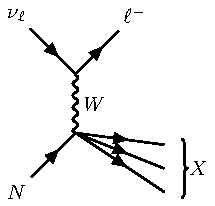
\includegraphics[width=0.4\linewidth]{images/neutrino-nucleon-dis.pdf}
\caption{Диаграмма Фейнмана, соответствующая глубоконеупругому взаимодействию нейтрино с нуклоном через обмен $W$-бозоном. Существует аналогичная диаграмма с обменом $Z$-бозоном, при этом $\ell^- \to \nu$.}
\label{fig:DIS}
\end{figure}

Определим кинематические переменные. Обозначим 4-импульсы: 
$k = (E_\nu, \bm{k})$ — нейтрино, 
$k' = (E_\ell, \bm{k}')$ — лептона в конечном состоянии, 
$p = (M, \bm{0})$ — нуклона в лабораторной системе, 
$p'$ — адронной системы, 
$q = k - k' = p' - p$ — переданный 4-импульс.

Для описания глубоконеупругого рассеяния используется три независимые кинематические переменные: \( Q^2 \equiv -q^2\) и переменные Бьёркена \( x \) и \( y \).
\begin{equation}
  Q^2 \approx 2(E_\nu E_\ell - \bm{k} \cdot \bm{k}') \approx 4E_\nu E_\ell \sin^2\!\frac{\theta}{2},
\end{equation}
где \( \theta \) — угол рассеяния лептона в лабораторной системе. В области глубоконеупругого рассеяния \( Q^2 > 0 \).

Переменные Бьёркена:
\begin{equation}
  x = \frac{Q^2}{2(p \cdot q)}, 
  \qquad 
  y = \frac{p \cdot q}{p \cdot k}.
\end{equation}

Кроме того, полезно использовать:
\begin{enumerate}
  \item \( W^2 = (p + q)^2 = M^2 + 2(p \cdot q) - Q^2 \) — инвариантный квадрат массы адронной системы;
  \item \( s = (k + p)^2 \) — квадрат полной энергии в системе центра масс нейтрино-нуклон.
\end{enumerate}

\subsection{Дифференциальное сечение}

Сечение нейтрино–нуклонного глубоконеупругого рассеяния можно записать в универсальной форме:
\begin{equation}
  \frac{d^2 \sigma_{\text{DIS}}}{dx\,dy} =
  \frac{G_F^2 M E_\nu}{\pi \bigl(1 + Q^2/M_W^2\bigr)^2}
  \sum_{i=1}^{5} A_i(x, y, E_\nu)\, F_i(x, Q^2),
  \label{eq:xsec_general}
\end{equation}
где \( G_F \) — константа Ферми, \( M \) — масса нуклона, \( E_\nu \) — энергия нейтрино, \( Q^2 \) — квадрат переданного импульса, \( F_i(x, Q^2) \) — структурные функции, а \( A_i(x, y, E_\nu) \) — известные кинематические коэффициенты, зависящие от энергии и переменных Бьёркена \( x \) и \( y \).

Структурные функции \( F_i(x, Q^2) \) выражаются через партонные распределения и содержат информацию о внутренней структуре нуклона. Конкретная форма коэффициентов \( A_i \) зависит от свойств начальных частиц, включая их поляризацию. Некоторые подробности приведены в приложении~\ref{app:structure_functions}.

На рис.~\ref{fig:xsec_2d} представлены дважды дифференциальные сечения $\frac{d^2\sigma}{dx\,dy}$ для взаимодействия мюонного нейтрино с протоном через обмен бозоном $W$, рассчитанные при различных энергиях нейтрино и фиксированных значениях переменной $y$. Характерной особенностью этих графиков является то, что с ростом энергии основная часть сечения смещается в область всё меньших значений переменной Бьёркена $x$. Это отражает фундаментальную особенность глубоко-неупругого рассеяния: при больших $Q^2$ всё больший вклад в сечение начинают вносить морские кварки и антикварки.

\begin{figure}[!h]
\centering
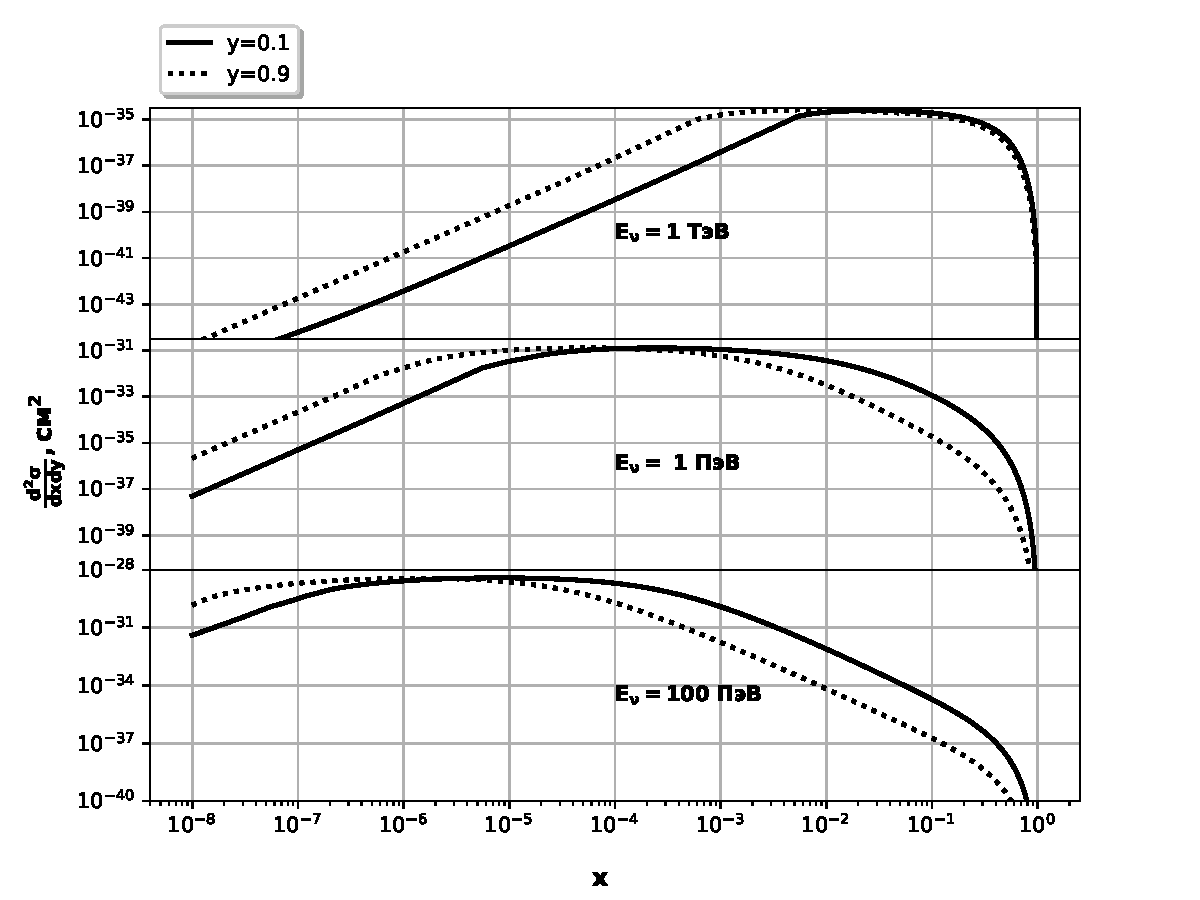
\includegraphics[width=\linewidth]{images/NuProp/xs_vs_xCT18ZNNLO_cc_12_proton.pdf}
\caption{Дважды дифференциальные сечения для рассеяния мюонного нейтрино на протоне за счёт заряженного тока в зависимости от переменной Бьёркена $x$ при различных энергиях нейтрино и фиксированных значениях переменной $y$.}
\label{fig:xsec_2d}
\end{figure}

Вклад малых бъёркеновских $x$ в полное сечение исследуется в разделе~\ref{sec:dis_reliability}.

\subsection{Программный пакет \texttt{nudisxs}}

\texttt{nudisxs}~\cite{nudisxs2022} — программный модуль на языке Python~3, предназначенный для вычисления сечений нейтрино–нуклонного взаимодействия в области глубоконеупругого рассеяния по формуле~\eqref{eq:xsec_general}. 
Его вычислительное ядро основано на пакете \texttt{XsDis}, написанном на языке Fortran В.~А.~Наумовым и К.~С.~Кузьминым (см., например,~\cite{nudisxs2022}). 
В отличие от исходной версии, рассчитанной на фиксированный набор партонных функций, \texttt{nudisxs} поддерживает динамическую загрузку партонных распределений из библиотеки \texttt{LHAPDF6}~\cite{aartsenLHAPDF2020}.

Модуль позволяет вычислять дважды дифференциальные сечения по переменным Бьёркена~$x$ и~$y$, дифференциальные сечения по одной переменной и полные сечения взаимодействия в широком диапазоне энергий — от сотен~МэВ до~$10^{15}$~ГэВ. 
Он предназначен для задач нейтринной астрофизики и моделирования событий в нейтринных телескопах и может быть легко интегрирован в существующие исследовательские проекты.

Реализация использует библиотеки \texttt{NumPy}~\cite{2020NumPy-Array}, \texttt{SciPy}~\cite{2020SciPy-NMeth} и \texttt{vegas}~\cite{lepageVegas2021} для многомерного Монте–Карло интегрирования, что обеспечивает высокую производительность и удобство при численном анализе и тестировании. 
%

Логическая архитектура пакета \texttt{nudisxs} показана на рис.~\ref{fig:nudisxs1}. 
Основой расчётов является загрузка партонных функций из библиотеки \texttt{LHAPDF6}, используемых для построения структурных функций $F_i(x, Q^2)$, входящих в выражение~\eqref{eq:xsec_general}. 
Пользовательский интерфейс реализован в модуле \texttt{dis}, где задаются тип лептона (нейтрино или антинейтрино), мишень (протон, нейтрон или изоскаляр), энергия нейтрино, минимальное значение $Q^2$, а также выбранный набор партонных распределений и параметров модели. 
Вычисление дважды дифференциальных сечений для заряженного и нейтрального токов выполняют модули \texttt{xs\_cc} и \texttt{xs\_nc}. 
Часть исходного кода, написанного на~Fortran, доступна через интерфейс \texttt{f2py} и обеспечивает быстрые, проверенные временем вычисления ключевых выражений. 
Интерполяция партонных распределений, построение структурных функций и численные процедуры реализованы средствами \texttt{SciPy}.

\begin{figure}[!h]
\centering
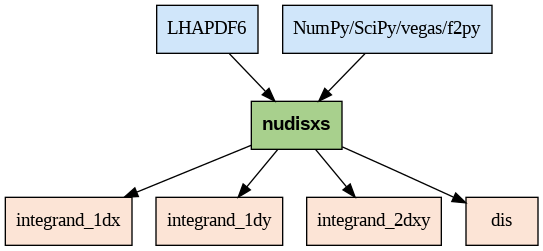
\includegraphics[width=\linewidth]{images/nudisxs_diagram.png}
\caption{Структура программного пакета \texttt{nudisxs} и его зависимости.}
\label{fig:nudisxs1}
\end{figure}

Пакет \texttt{nudisxs} распространяется через платформу \texttt{PyPI} как открытое программное обеспечение. 
Он легко устанавливается и интегрируется в существующие симуляционные цепочки. 
В рамках настоящей работы \texttt{nudisxs} использован для расчёта всех сечений, показанных на рис.~\ref{fig:xsec_2d}–\ref{fig:xsec_total}.

\section{Достоверность партонной модели при ПэВ-энергиях}
\label{sec:dis_reliability}
На рис. (\ref{fig:xQ2_PDG}) приведена исследованная область в экспериментах на коллайдерах:   БАК (LHC), Теватрон, HERA, а также в экспериментах с неподвижной мишенью. В области малых $x\lesssim 10^{-6}$ экспериментальные измерения практически отсутствуют. Между тем, с ростом энергии взаимодействия нейтрино, вклад именно малых $x$ в сечение взаимодействия становится доминирующим. Выход в неисследованную область с необходимостью требует использования экстраполяции, что является источником дополнительной систематической неопределённости. 
\begin{figure}[!h]
\centering
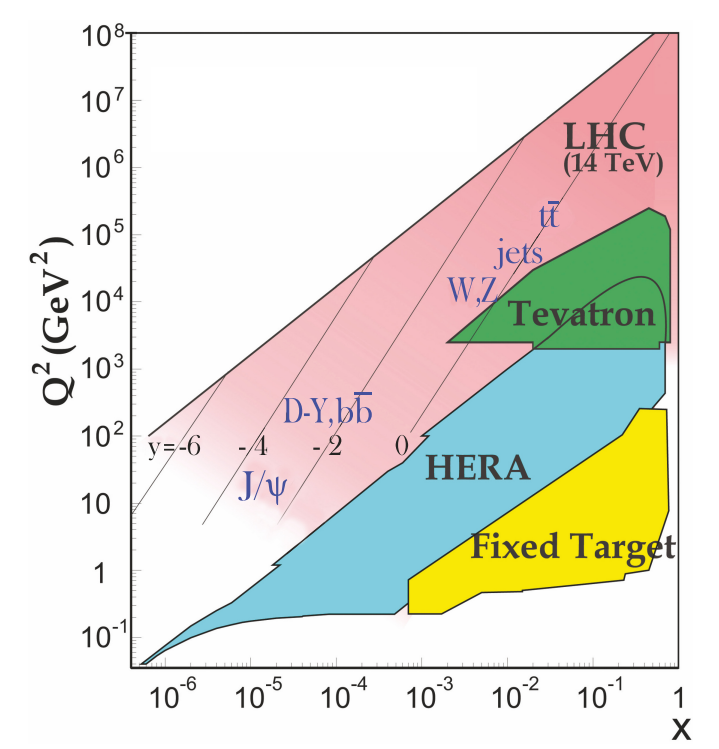
\includegraphics[width=0.8\linewidth]{images/NuProp/reald}
\caption{Кинематические области в $x$ и $Q^2$, исследованные в экспериментах с неподвижной мишенью и на коллайдерах. Рисунок из \cite{ParticleDataGroup:2024cfk}.}
\label{fig:xQ2_PDG}
\end{figure}

\subsection{Вклад экспериментально недоступной области}
Для иллюстрации, на рис.~\ref{fig:diff_xsec_100PeV} приведено дважды дифференциальное нормированное сечение
\[
\frac{1}{\sigma(E_\nu)}\frac{d^2\sigma(E_\nu,x,Q^2)}{dx\,dQ^2}
\] 
как функция переменных $x$ и $Q^2$ при энергии нейтрино $E_{\nu} = 100$ ПэВ. $\sigma(E_\nu)$ - полное сечение глубоконеупругого взаимодействия нейтрино с нуклоном при фиксированной энергии нейтрино. 

На рисунке также приведена заштрихованная область, качественно отражающая экспериментально исследованную область, представленную на рис.~\ref{fig:xQ2_PDG}.
\begin{figure}[!h]
\centering
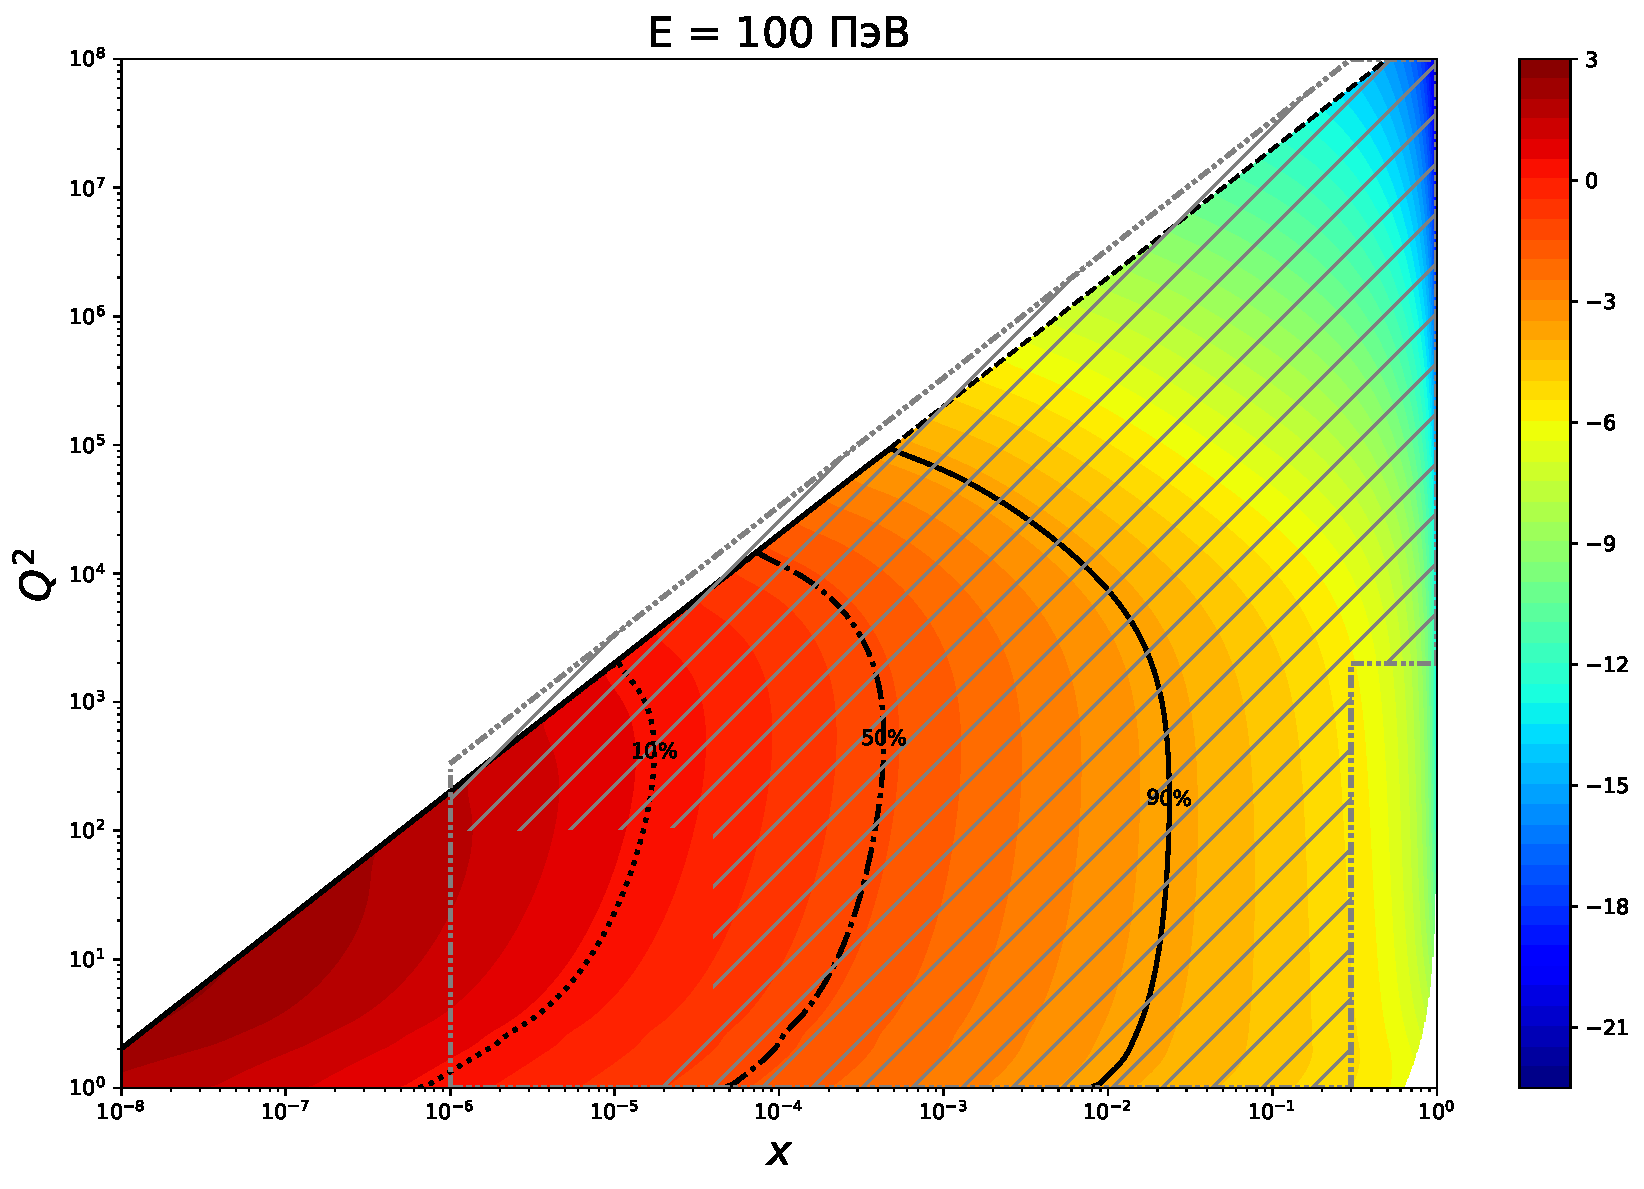
\includegraphics[width=0.8\linewidth]{images/NuProp/cdfxq2_cc_proton_CT18ZNNLO_14_100000000.pdf}
\caption{Дважды дифференциальное ормированное сечение $\frac{1}{\sigma(E_\nu)}\frac{d^2\sigma(E_\nu,x,Q^2)}{dx\,dQ^2}$ как функция $x$ и $Q^2$ для энергии нейтрино $E_{\nu} = 100$ ПэВ. Использованы партонные распределения CTEQ15\cite{ncteq15}.}
\label{fig:diff_xsec_100PeV}
\end{figure}

В области $x\lesssim 10^{-6}$, где экспериметальные данные отсутствуют, $\frac{1}{\sigma(E_\nu)}\frac{d^2\sigma(E_\nu,x,Q^2)}{dx\,dQ^2}$ максимально.  Пунктирные линии в пространстве $x,Q^2$ на рисунках указывают области, где сечения насыщаются до определенного уровня: $10\%$, $50\%$, $90\%$. Можно сделать заключение, что вклад области $x\lesssim 10^{-6}$ порядка $5\%$. В приложении~\ref{sec:examples_extrapolated_region} приведены еще два примера аналогичных распределений для энергий нейтрино 1 ТэВ и 1 ПэВ. 

Более простой способ оценки заключается в том, чтобы пренебречь сложной зависимостью двумерной области $x,Q^2$, в которой существуют экспериментальные измерения, а сосредоточиться только на главной в данном контексте переменной - $x$ Бьёркена. Определим отношение: 
\begin{equation}
\frac{1}{\sigma(E_\nu)}\int\limits_{x}^1\,\frac{d\sigma(E_\nu,x')}{dx'}dx',
\label{eq:CDF_x}
\end{equation}
где 
\[
\frac{d\sigma(E_\nu,x)}{dx} = \int\limits_0^{1}dy\,\frac{d^2\sigma(E_\nu,x,y)}{dx\,dy}.
\]
На рис.~\ref{fig:CDF_x} приведена функция~\eqref{eq:CDF_x} в зависимости от $x$ и $Q^2$ для треё значений энергии нейтрино $E_{\nu}= $ 1 ТэВ, 1 ПэВ, 100 ПэВ.
\begin{figure}[!h]
\centering
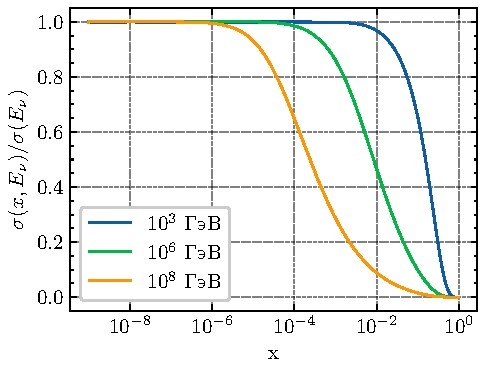
\includegraphics[width=0.8\linewidth]{images/NuProp/cdfxy_plot_CT18ZNNLO_14.pdf}
\caption{Функция $\int\limits_{x}^1\,\frac{1}{\sigma(E_\nu)}\frac{d\sigma(E_\nu,x')}{dx'}dx'$ в зависимости от $x$ и $Q^2$ для треё значений энергии нейтрино $E_{\nu}= $ 1 ТэВ, 1 ПэВ, 100 ПэВ. Использованы партонные распределения CTEQ15\cite{ncteq15}.}
\label{fig:CDF_x}
\end{figure}


\subsection{Полное сечение и его вариация от параметризации}
Из первых принципов довольно сложно оценить вклад неисследованной области в величину полного сечения. Косвенный метод - использовать вариацию в полном сечении при использование различных теоретических параметризаций.  На рис.~\ref{fig:xsec_total} показана зависимость полного сечения взаимодействия мюонного нейтрино на нуклоне от энергии для различных партонных распределений. Также, приведена вариация полного сечения, связанная с использовании разных наборов партонных распределений. Можно сделать вывод о том, что оценка на уровне $5\%$ вариации отвечает наблюдению из предыдущего раздела.

\begin{figure}[!h]
\centering
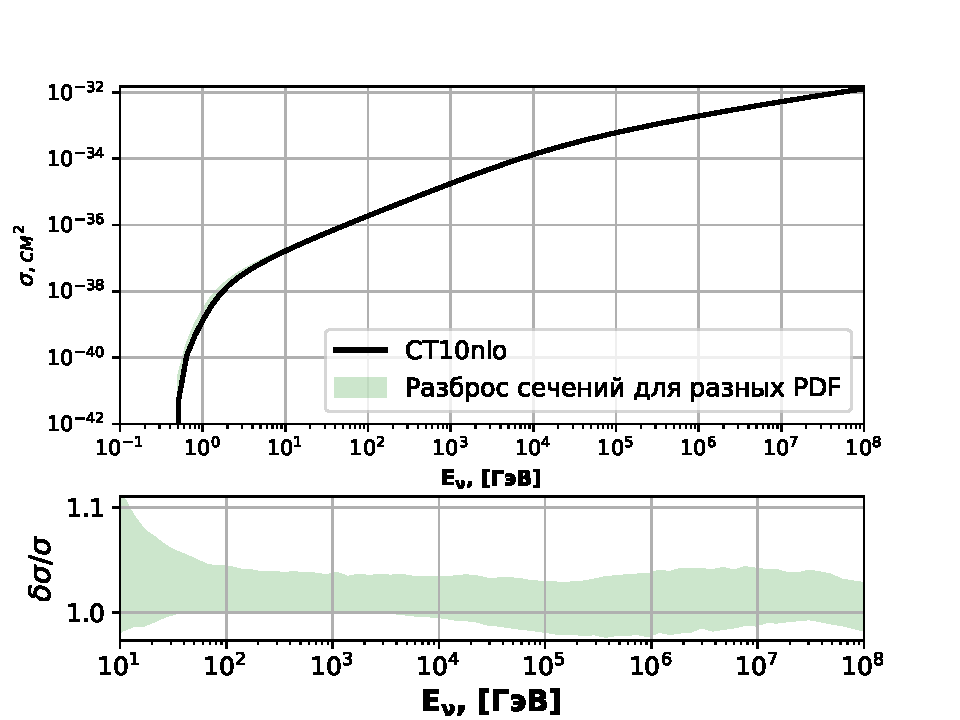
\includegraphics[width=\linewidth]{images/NuProp/xs_vs_enu.pdf}
\caption{Полные сечения взаимодействия мюонного нейтрино на нуклоне в зависимости от энергии $E_\nu$ для партонных распределений \texttt{CT10nlo}. Полоса отвечает вариации полного сечения при использовании других наборов партонных распределений (\texttt{CT18ZNNLO}, \texttt{nCTEQ15}, \texttt{TUJU19\_nlo}).} 
\label{fig:xsec_total}
\end{figure}

\section{Расчёт прохождения нейтрино через Землю}
\label{sec:zfactor}
В работе используется модель PREM для описания плотности вещества Земли (см. приложение~\ref{sec:prem}). Расчёт глубины 
\[
X=\int\limits_\text{траектория}\rho(\ell) d\ell
\]
осуществляется численным интегрированием плотности вдоль траектории нейтрино.

\subsection{$\mathcal{Z}$-факторный метод}

$\mathcal{Z}$-фактор представляет собой поправку к затуханию потока нейтрино, учитывающую регенерацию за счёт нейтрального тока. Метод предложен и подробно описан в работе~\cite{naumov1999} и базируется на решении следующего уравнения переноса нейтрино:
\begin{equation}
\frac{\partial F_{\nu}(X,E_\nu)}{\partial X} = \frac{1}{\lambda_{\nu}(E_\nu)}\left[ \int\limits_0^1\frac{dy}{1-y}\Phi_{\nu}(y,E_\nu) F_{\nu}(X,E_y) - F_{\nu}(X,E_\nu) \right],
\end{equation}
где $F_{\nu}(X,E_\nu)$ — поток нейтрино после прохождения глубины $X$, $E_y = E_\nu/(1-y)$, 
\[
\lambda^{-1}_{\nu}(E_\nu) = \sum\limits_{T\in \{n,p,e\}}n_T\sigma_{\nu T}^{tot}(E)
\] 
- пропорционально полному сечению взаимодействия нейтрино с веществом, а $\Phi_{\nu}(y,E)$ — распределение по передаче энергии, определяемое следующей формулой:
\begin{equation}
    \Phi_{\nu}(y,E_\nu) = \frac{\sum\limits_{T\in \{n,p,e\}}n_T\frac{d\sigma_{\nu T}}{dy}(y,E_y)}{\sum\limits_{T\in \{n,p,e\}}n_T\sigma_{\nu T}(E_\nu)}.
\end{equation}
В этих формулах $n_T$ число мишеней на грамм вещества.

Искомое решение имеет вид:
\begin{equation}
F_{\nu}(X,E_\nu) = F^{0}_{\nu}(E_\nu)\exp\left(-\frac{x}{\Lambda_{\nu}(X,E_\nu)}\right),
\end{equation}
где 
\begin{equation}
\Lambda_{\nu}(X,E_\nu) = \frac{\lambda_{\nu}(E_\nu)}{1 - \mathcal{Z}_{\nu}(X,E_\nu)}.
\end{equation}

Решение уравнения для $\mathcal{Z}_{\nu}(X,E_\nu)$ реализуется итерационно, начиная с $\mathcal{Z}^{(0)}$ и строя следующие приближения по схеме:
\begin{equation}
\mathcal{Z}^{(n+1)}_{\nu}(X,E_\nu) = \int\limits_0^X dX' \int\limits_0^1 dy\,\eta_{\nu}(y,E_\nu)\Phi_{\nu}(y,E_\nu)\exp\left[ -X'D^{(n)}_{\nu}(X',E_\nu,E_y) \right],
\end{equation}
где $\eta_{\nu}(y,E_\nu)$ — весовой фактор, определяемый формой начального спектра. Точное выражение для $\eta_{\nu}(y,E_\nu)$ имеет следующий вид: 
\begin{equation}
    \eta_{\nu}(y,E_\nu) = \frac{F^0_{\nu}(E_y)}{(1-y)F^0_{\nu}(E_\nu)}.
\end{equation}
Выражение для фактора $D^{(n)}_{\nu}(x, E_\nu, E_y)$ имеет следующий вид:
\begin{equation}
    D^{(n)}_{\nu}(X, E_\nu, E_y) = \frac{1-\mathcal{Z}_{\nu}^{(n)}(X, E_y)}{\lambda(E_y)} - \frac{1-\mathcal{Z}_{\nu}^{(n)}(X, E_\nu)}{\lambda(E_\nu)}.
\end{equation}
Решение уравнения переноса для потока нейтрино учитывает как исчезновение нейтрино за счёт заряженного тока, так и эффект регенерации от нейтрального тока. 

\subsection{Непрозрачность Земли}
Иллюстрация решения $\mathcal{Z}$-факторным методом приведена на  рис. (\ref{EF2}). Здесь показано отношение потока нейтрино $F_\nu(X(\theta),E_\nu)$  после прохождения вещества Земли к потоку $F_\nu^0(X(\theta),E_\nu)$ на поверхности Земли. Это  отношение можно считать приближением к вероятности прохождения нейтрино.
\begin{figure}[!h]
\centering
\includegraphics[width=0.8\linewidth]{images/NuProp/rzf_2dxsTUJU19_nlo_2_1.png}
\caption{Вероятность прохождения нейтрино сквозь Землю в зависимости от энергии и зенитного угла, измеряющегося относительно детектора.}
\label{EF2}
\end{figure}
Тёмно-синия область на рис.~(\ref{EF2}) отвечает ситуации когда Земля становится практически непрозрачной для нейтрино.

Для вычисления графика~(\ref{EF2}) использовалась следующая модель спектра нейтрино:
\begin{equation}
    F_{\nu}^{0}(E) = K\left(\frac{E_0}{E}\right)^{\gamma+1} (1+E_0/E)^{-\alpha},%\phi\left(\frac{E}{E_{cut}}\right),
\end{equation}
с параметрами $\gamma = 1$ и $\alpha = 0.5$. 
% $\phi_{cut}(t)$ - некоторая функция, предназначенная для обрезания потоков при энергиях выше некоторого порога. В настоящей работе использована:
% \begin{equation}
%     \phi(t) = (1+\tan(\pi t/2))^{-1}
% \end{equation}

\section{Программный пакет \texttt{NuPropagator}}

\subsection{Общее описание и структура}

Пакет \texttt{NuPropagator}~\cite{nupropagator2022} представляет собой модуль для моделирования прохождения потоков нейтрино через вещество, в частности через Землю, с учётом взаимодействий по заряженному и нейтральному токам. Он реализует итеративный метод на основе $\mathcal{Z}$-фактора, что позволяет учитывать регенерацию нейтрино при рассеянии на нуклонах. Пакет написан на языке \texttt{Python3} и поддерживается через платформу \texttt{PyPI}, что обеспечивает его доступность и простоту интеграции в существующие симуляционные цепочки.

\begin{figure}[!h]
\centering
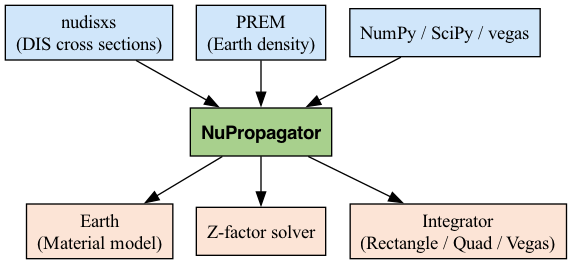
\includegraphics[width=\linewidth]{images/nupropagator_diagram.png}
\caption{Структура программного пакета \texttt{nupropagator} и его зависимости.}
\label{fig:nupropagator1}
\end{figure}

\subsection{Физическая модель}

Пакет \texttt{NuPropagator} использует следующие физические компоненты:
\begin{itemize}
  \item модель плотности Земли (PREM);
  \item сечения взаимодействия нейтрино с нуклонами, предоставляемые пакетом \texttt{nudisxs};
  \item итерационный метод Z-фактора для расчёта эволюции нейтринного спектра.
\end{itemize}

\subsection{Модель плотности Земли и расчёт толщины}

В качестве модели плотности используется Предварительная эталонная модель Земли (PREM)~\cite{dziewonskiPREM1981}, которая предполагает сферическую симметрию и описывает плотность, давление и другие параметры как функции радиуса. Плотность в модели представлена на рис.~\ref{PREM}.

\begin{figure}[!h]
\centering
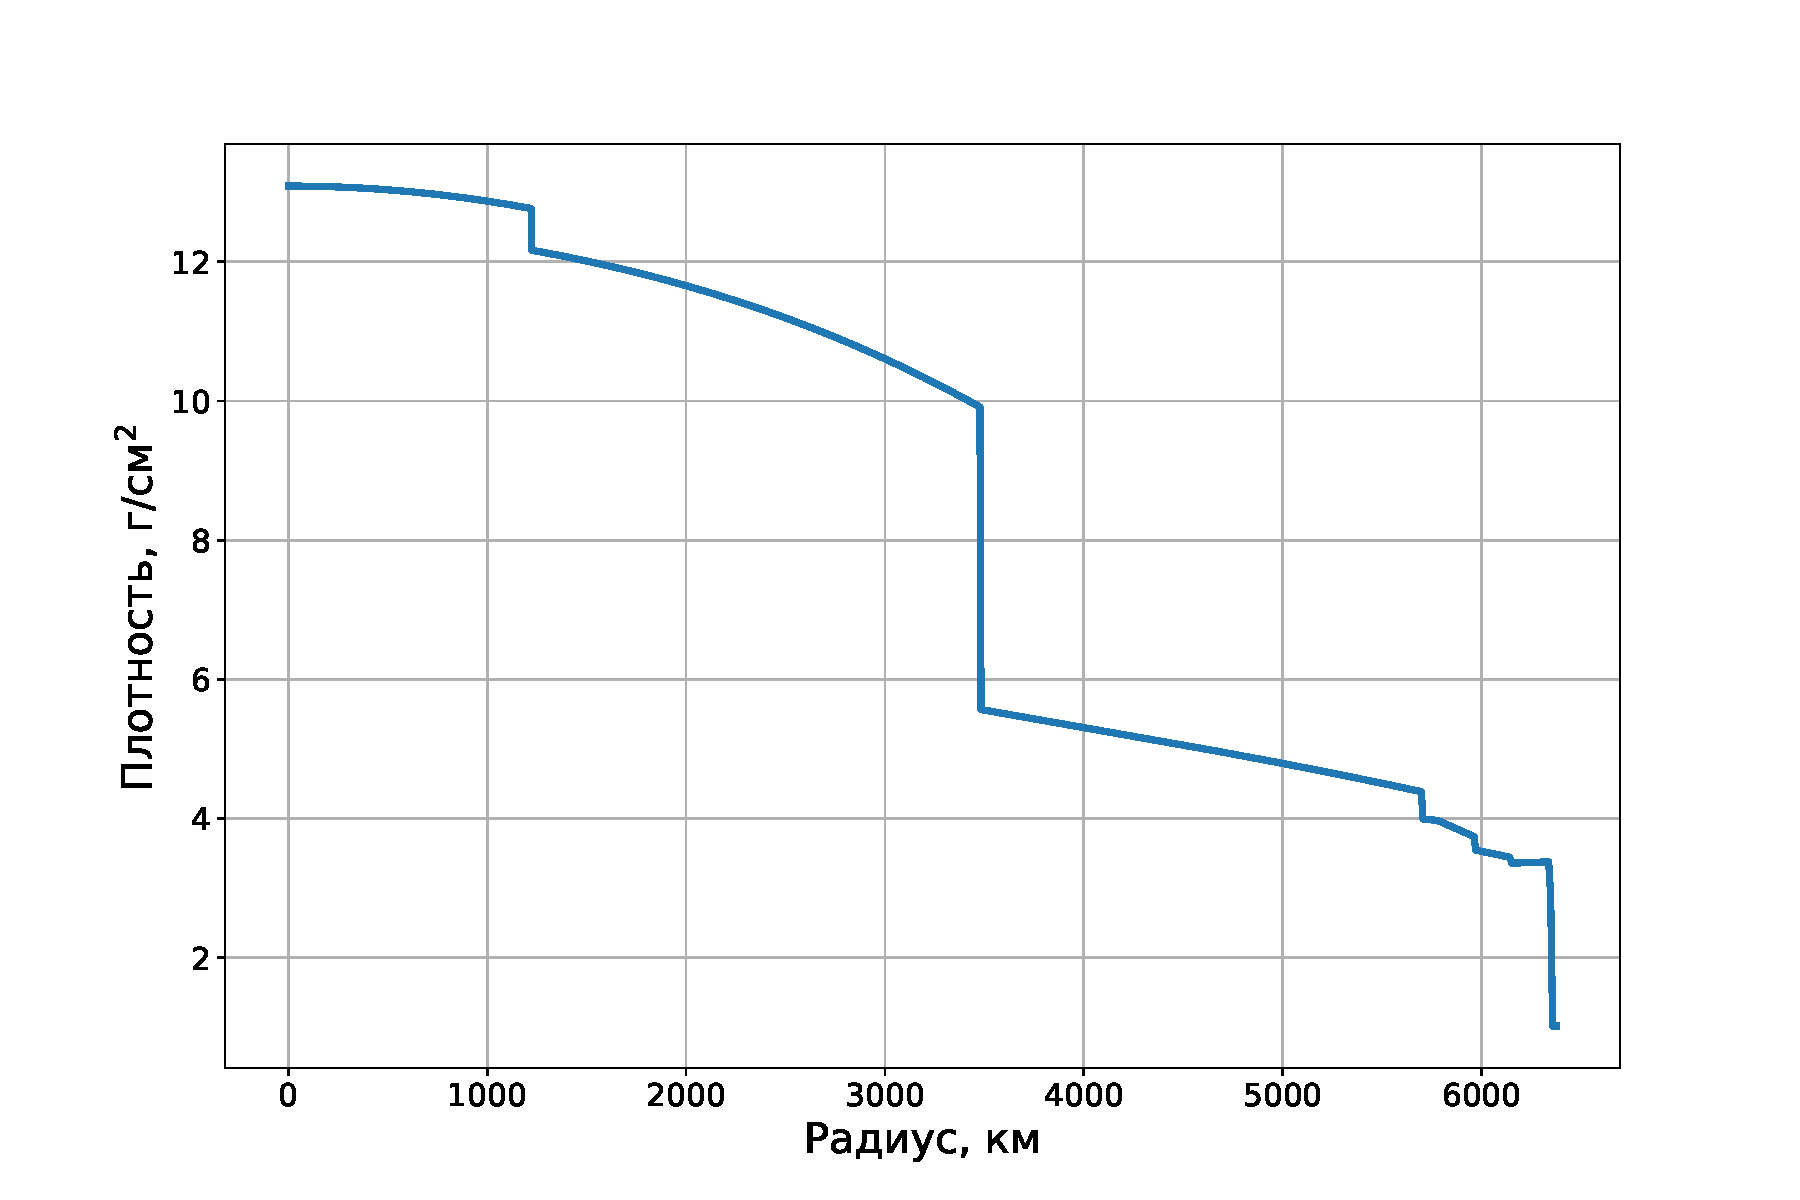
\includegraphics[width=\linewidth]{images/NuProp/PREM.pdf}
\caption{Плотность вещества в модели Земли PREM.}
\label{PREM}
\end{figure}

Расчёт толщины вещества, проходимого нейтрино, осуществляется интегрированием плотности вдоль траектории. Поддерживаются несколько численных методов: метод прямоугольников, квадратурный метод \texttt{quad} из \texttt{SciPy}, и метод Монте-Карло \texttt{vegas}. Изотопный состав вещества задаётся в модуле Earth пакета \texttt{NuPropagator}.

\subsection{Метод Z-фактора}

Z-фактор представляет собой поправку к затуханию потока нейтрино, учитывающую регенерацию за счёт нейтрального тока. Метод подробно описан в работе~\cite{naumov1999} и базируется на решении следующего уравнения переноса нейтрино:
\begin{equation}
\frac{\partial F_{\nu}(x,E)}{\partial x} = \frac{1}{\lambda_{\nu}(E)}\left[ \int\limits_0^1\frac{dy}{1-y}\Phi_{\nu}(y,E) F_{\nu}(x,E_y) - F_{\nu}(x,E) \right],
\end{equation}
где $F_{\nu}(x,E)$ — поток нейтрино после прохождения толщины $x$, $E_y = E/(1-y)$, $\lambda{E}$ - полное сечение взаимодействия нейтрино с веществом, а $\Phi_{\nu}(y,E)$ — распределение по передаче энергии, определяемое следующей формулой:
\begin{equation}
    \Phi_{\nu}(y,E) = \frac{\sum\limits_{T\in \{n,p,e\}}N_T\frac{d\sigma_{\nu T}}{dy}(y,E_y)}{\sum\limits_{T\in \{n,p,e\}}N_T\sigma_{\nu T}(E)}
\end{equation}

Предполагаемое решение имеет вид:
\begin{equation}
F_{\nu}(x,E) = F^{0}_{\nu}(E)\exp\left(-\frac{x}{\Lambda_{\nu}(x,E)}\right),
\end{equation}
где 
\begin{equation}
\Lambda_{\nu}(x,E) = \frac{\lambda_{\nu}(E)}{1 - \mathcal{Z}_{\nu}(x,E)}.
\end{equation}

\subsection{Итерационный метод и его реализация}

Решение уравнения для $\mathcal{Z}_{\nu}(x,E)$ реализуется итерационно, начиная с $\mathcal{Z}^{(0)}$ и строя следующие приближения по схеме:
\begin{equation}
\mathcal{Z}^{(n+1)}_{\nu}(x,E) = \int\limits_0^x dx' \int\limits_0^1 dy\,\eta_{\nu}(y,E)\Phi_{\nu}(y,E)\exp\left[ -x'D^{(n)}_{\nu}(x',E,E_y) \right],
\end{equation}
где $\eta_{\nu}(y,E)$ — весовой фактор, определяемый формой начального спектра. Точное выражение для $\eta_{\nu}(y,E)$ имеет следующий вид: 
\begin{equation}
    \eta_{\nu}(y,E) = \frac{F^0_{\nu}(E_y)}{(1-y)F^0_{\nu}(E)}.
\end{equation}
Выражение для фактора $D^{(n)}_{\nu}(x, E, E_y)$ имеет следующий вид:
\begin{equation}
    D^{(n)}_{\nu}(x, E, E_y) = \frac{1-\mathcal{Z}_{\nu}^{(n)}(x, E_y)}{\lambda(E_y)} - \frac{1-\mathcal{Z}_{\nu}^{(n)}(x, E)}{\lambda(E)}
\end{equation}
Реализация учитывает как исчезновение нейтрино за счёт заряженного тока, так и эффект регенерации от нейтрального тока. Конечная плотность потока описывается экспоненциальным затуханием с учётом эффективной длины пробега:
\begin{equation}
P(E,x) = \exp(-x/\lambda_{\nu}(E)), \quad x = \int\rho(l)\,dl.
\end{equation}
\subsection{Сравнение с другими программными пакетами}
 Проведем сравнение результатов, полученных с помощью двух програмнных пакетов: \texttt{nuFATE}~\cite{Vincent_2017} и \texttt{nupropagator}. Будем сравнивать потоки мюонного нейтрино, приходящих под разными углами после прохождения через землю в некоторой точке, находящейся на глубине 1 км от поверхности Земли. В качестве нейтринного потока на поверхности земли был использован степенной поток $E^{-2}$.
\begin{figure}[!h]
\centering
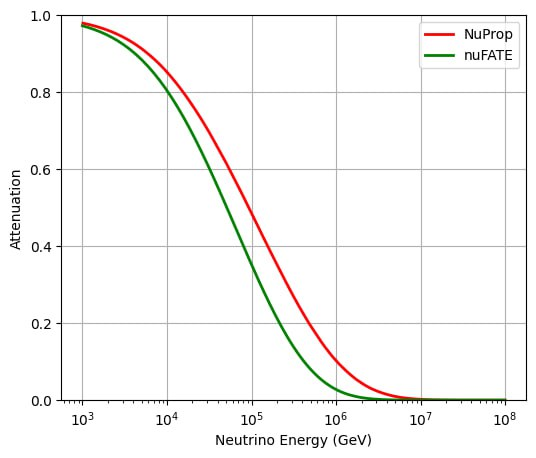
\includegraphics[width=\linewidth]{images/NuProp/compare_fluxes.jpg}
\caption{Сравнение потоков, полученных с помощью \texttt{nuFATE} и \texttt{Nupropagator} для разных углов прилета нейтрино.}
\label{fig:flux_compare}
\end{figure}
Как можно видеть из рис.~\ref{fig:flux_compare} результаты находятся в полном согласии. 



\subsection{Дополнительные возможности}
% (Оставьте место для дополнения при необходимости)

\subsection{Интеграция с другими модулями}
% (Добавьте описание связей с другими компонентами симуляционного фреймворка)

\subsection{Поддержка и установка}

Пакет \texttt{NuPropagator} доступен через \texttt{PyPI} и может быть установлен командой:
\begin{verbatim}
pip install nupropagator
\end{verbatim}
Полная документация доступна на странице проекта, включающей примеры использования и описание API.

\section{Нейтринная томография Земли}
\label{sec:tomography}
В этом разделе рассматривается возможность уточнения распределения плотности Земли с помощью нейтрино сверхвысоких энергий.  
В настоящее время сведения о внутренней структуре и плотности Земли получены главным образом из сейсмологических наблюдений, в частности в рамках модели PREM (Preliminary Reference Earth Model)~\cite{dziewonskiPREM1981}.

Идея использовать нейтринные осцилляции при энергиях порядка нескольких ГэВ для реконструкции плотности Земли активно обсуждается в контексте современных нейтринных детекторов, таких как DUNE, ORCA и PINGU~\cite{winterTomography2013,akhmedovTomography2006}.  
Однако такой подход сталкивается с серьёзными экспериментальными трудностями: требуется (i) высокая точность реконструкции энергии, (ii)направления приходящих нейтрино, (iii) большая масса детектора, (iv) эффективное подавление фоновых событий. Все эти требования  довольно сложно удовлетворить практически для ГэВ-ных энергий нейтрино.

Альтернативный метод основан на эффекте поглощения нейтрино сверхвысоких энергий ($E_\nu \gtrsim 10$~ТэВ) при прохождении через Землю~\cite{gandhiAbsorption1998,franceTomography2019}.  
Поскольку сечение взаимодействия нейтрино растёт с энергией, поток таких частиц существенно ослабляется, особенно для траекторий, проходящих через ядро.  
Однако чувствительность этого метода, основанного только на поглощении (заряжённый ток), ограничена быстрым спадом числа наблюдаемых событий при росте энергии нейтрино.

В настоящей работе показано, что учёт \emph{регенерации потока} за счёт взаимодействий по нейтральному току существенно повышает чувствительность томографического метода.  
Нейтральные токи возвращают часть потока нейтрино на меньшие энергии, обеспечивая статистически значимое число событий даже при $E_\nu \gtrsim 1$~ПэВ.  
Таким образом, регенерация делает нейтринную томографию Земли практически осуществимой с использованием будущих крупномасштабных детекторов, таких как IceCube-Gen2 и KM3NeT.

\subsection{Важность регенерации}

При прохождении нейтрино сквозь Землю поток ослабляется вследствие взаимодействий по заряженному и нейтральному току.  
Заряжённый ток (\textit{CC}) отвечает за поглощение нейтрино: каждая реакция
\[
\nu_\ell + N \to \ell + X
\]
полностью удаляет нейтрино из пучка, и поток убывает экспоненциально:
\[
F_\nu(X(\theta_d),E_\nu) \propto 
e^{-N_A\,\sigma_{CC}(E)\,X(\theta_d)}, 
\qquad
X(\theta_d) = \int \rho(\ell)\, d\ell .
\]
Это создаёт базовую чувствительность к плотности Земли, однако число событий при этом быстро уменьшается с ростом энергии, и общая эффективность метода, основанного только на заряжённом токе, остаётся невысокой.

Нейтральный ток (\textit{NC}), напротив, не уничтожает нейтрино, а лишь понижает его энергию:
\[
\nu_\ell + N \to \nu_\ell' + X.
\]
Благодаря этому часть потока, потерянная на высоких энергиях, регенерируется на меньших энергиях, что приводит к заметному росту числа событий в детекторе.

Учёт \emph{регенерации нейтрино по нейтральному току} существенно повышает чувствительность нейтринной томографии Земли: без него поток нейтрино экспоненциально затухает, тогда как включение этого эффекта позволяет сохранять измеримый сигнал даже при $E_\nu \gtrsim 1$~ПэВ. 
Хотя влияние нейтрального тока на спектр нейтрино отмечалось и ранее, в настоящей работе этот эффект впервые детально рассмотрен с точки зрения его вклада в чувствительность методов томографии.

На рис.~\ref{EF1} показано, что вклад нейтрального тока становится доминирующим для нейтрино, проходящих через ядро Земли.

\begin{figure}[!h]
\centering
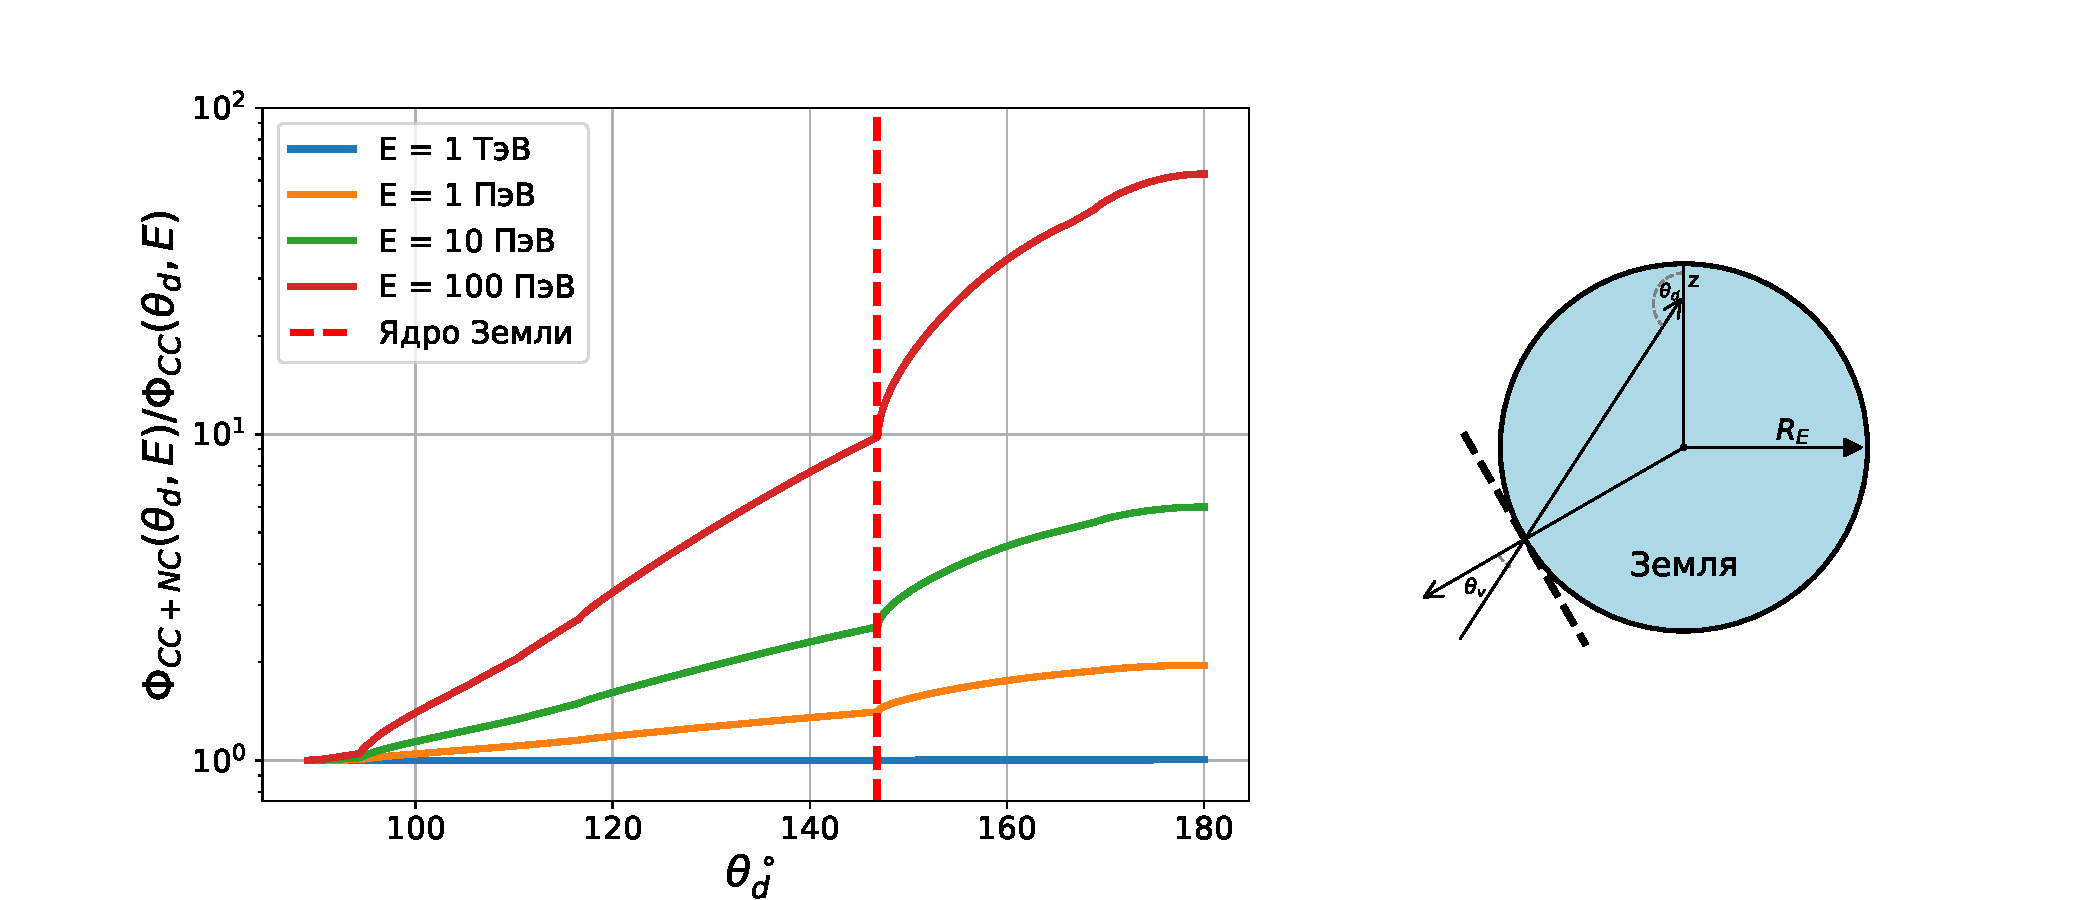
\includegraphics[width=\linewidth]{images/NuProp/rhh12zf_flux_index_CT18ZNNLO.pdf}
\caption{Влияние нейтрального тока на поток нейтрино в детекторе в зависимости от угла прихода $\theta_d$ и энергии $E_\nu$.  
Учёт нейтрального тока существенно увеличивает число регенерированных нейтрино, особенно для траекторий, проходящих через ядро Земли.}
\label{EF1}
\end{figure}

Таким образом, измеряя энергетические спектры нейтрино, прошедших через Землю, можно реконструировать распределение плотности вещества вдоль их траекторий — вплоть до ядра планеты.



% \subsection{Поглощение за счет нейтрального и заряженного токов}
% В конце зададимся вопросом, как изменяется показатель потока при прохождении нейтрино сквозь Землю за счёт разных взаимодействий. Предположим, что начальный и конечный потоки имеют форму 
% \begin{equation}
%     F_{in/fin}(E) = \Phi_0 E^{-\gamma_{in/fin}(E)}.
% \end{equation}
% На рис. (\ref{EF3}) можно видеть, что показатель потока начинает сильно изменяться при энергиях выше 10 ТэВ. Таким образом, для нейтрино высоких энергий, проходящих сквозь Землю, спектр будет сильно изменяться, поэтому количество событий для таких нейтрино будет сильно меньше ожидаемых. Нейтрино же, летящие сверху, не подвергнутся такому подавлению потока.    
% \begin{figure}[!h]
% \centering
% 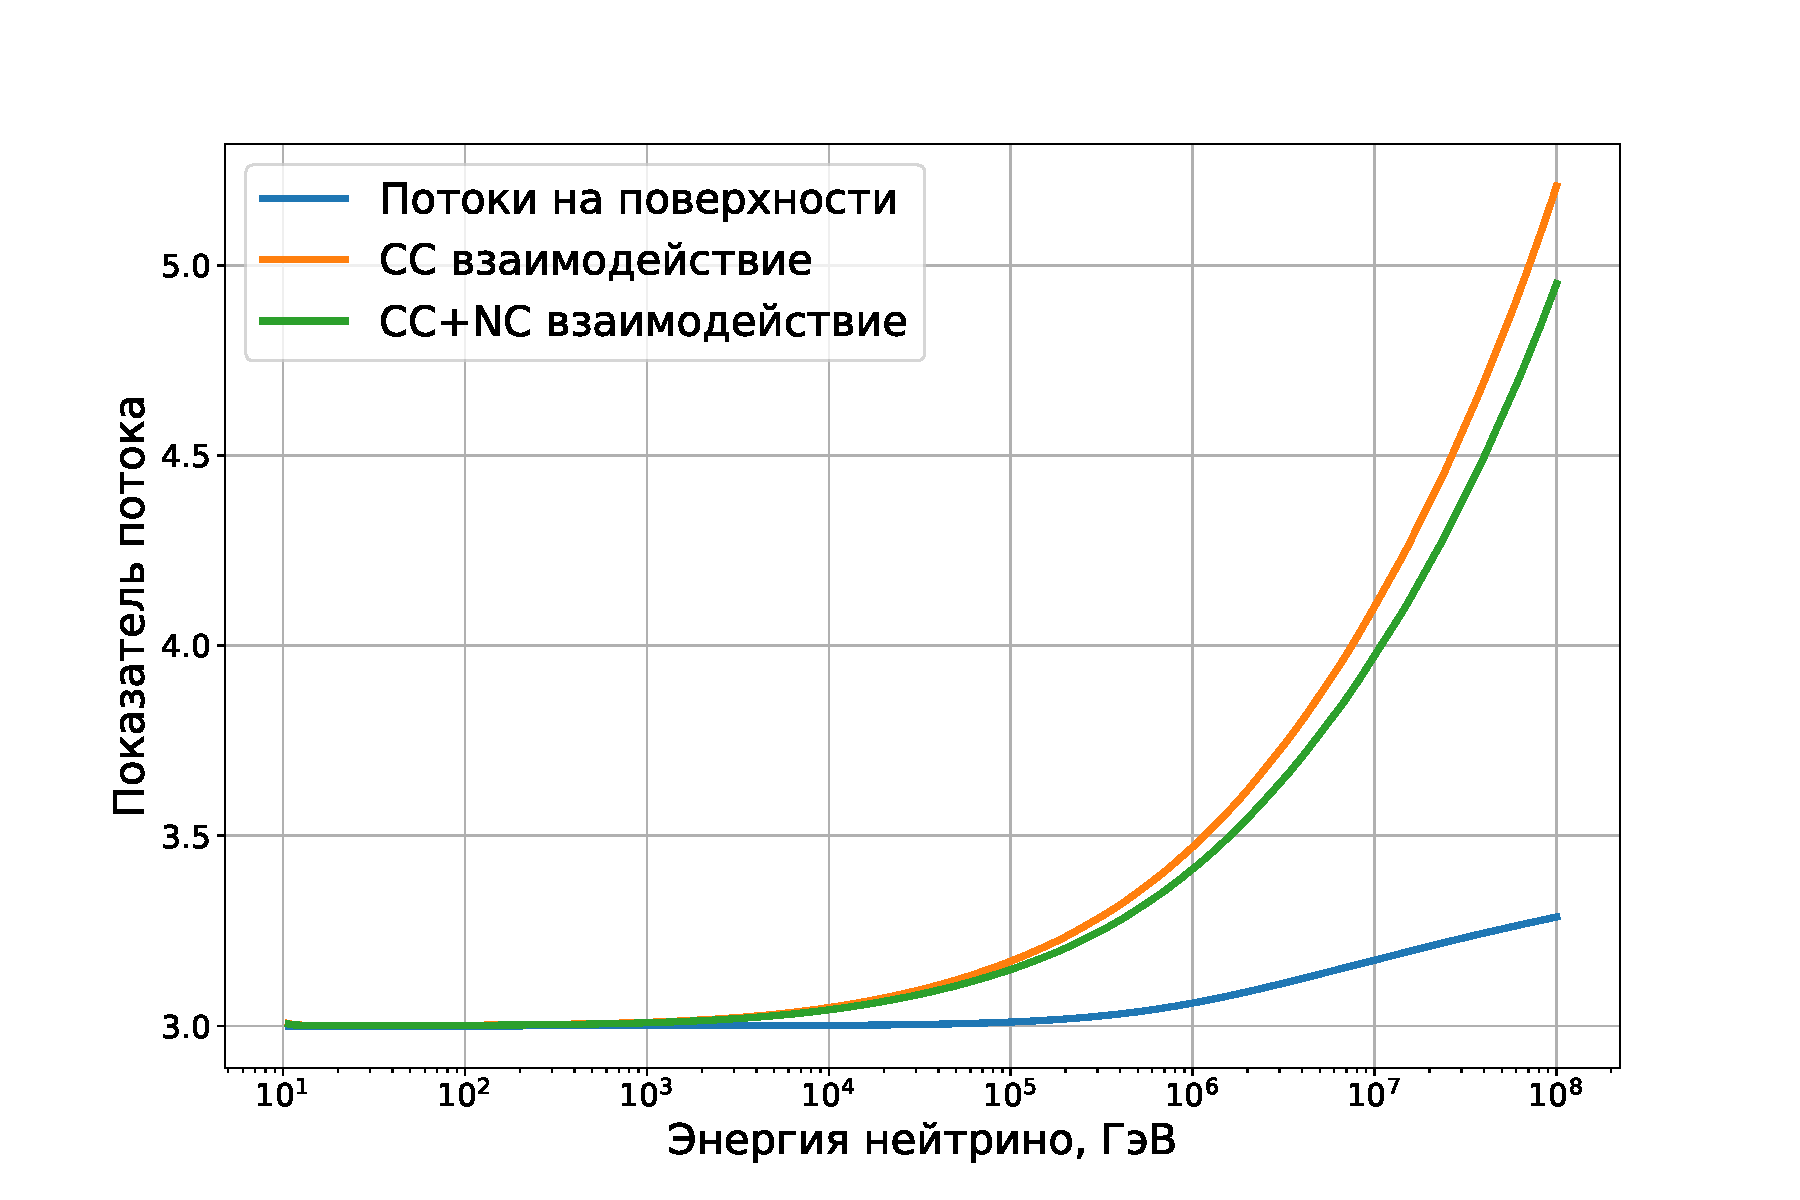
\includegraphics[width=1.1\linewidth]{images/NuProp/rzf_flux_index_CT18ZNNLO.pdf}
% \caption{Изменение показателя потока нейтрино для пучка, проходящего сквозь Землю в зависимости от энергии при учете разных типов взаимодействия.}
% \label{EF3}
% \end{figure}

\subsection{Статистический анализ}

Для количественной оценки чувствительности нейтринной томографии рассмотрим две гипотезы:  
\begin{itemize}
  \item $H_0$ — стандартная модель плотности Земли, соответствующая модели PREM~\cite{dziewonskiPREM1981};
  \item $H_1$ — альтернативные модели, описывающие возможные отклонения от PREM.
\end{itemize}

В качестве альтернативных гипотез рассматриваются три варианты распределения плотности:  
(1) модель с усреднённым ядром,  
(2) модель с линейным градиентом плотности в ядре,  
(3) модель с усреднёнными мантией и ядром.  

Гипотезы (2) и (3) рассматриваются в приложении~\ref{sec:appTomography}.

Сравнение гипотез проводится по статистике $\chi^2$, определяемой как
\begin{equation}
\label{eq:chi2_def}
\Delta\chi^2 = 2\sum_{i,j}
\left[
  N_{ij}^{(0)} - N_{ij}^{(1)} 
  + N_{ij}^{(1)}\ln\!\left(\frac{N_{ij}^{(1)}}{N_{ij}^{(0)}}\right)
\right],
\end{equation}
где $N^{(k)}_{ij}$ — ожидаемое число событий в интервале по энергии и углу для гипотезы $H_k$.  
Такое определение эквивалентно логарифму отношения правдоподобий (LLR) в предположении пуассоновской статистики и используется, например, в анализах коллабораций IceCube и ANTARES.

Для оценки статистической мощности метода рассчитывались полные числа событий в нейтринном телескопе объёмом $1~\text{км}^3$ за один год наблюдений при разных моделях плотности. На основе значений $\Delta\chi^2$ проверяется гипотеза $H_0$: большие значения статистики указывают на отличие рассматриваемой модели $H_1$ от PREM.

Для последующего анализа в качестве астрофизических потоков возьмем фит для диффузионного потока, рассчитанного коллаборацией IceCube ~\cite{Abbasi_2024}. Данные потоки рассчитаны в предположении степенного спектра на 1 флейвор нейтрино. В качестве атмосферных нейтринных потоков взяты потоки, полученные командой С. И. Синеговского~\cite{sinegovskaya2015}, рассчитанных на 1 флейвор нейтрино. В дальнейшем весь анализ будет проведён с учетом только мюонного флейвора ($\nu_{\mu}$ и $\bar{\nu}_{\mu}$).
  \begin{figure}[!h]
    \centering
    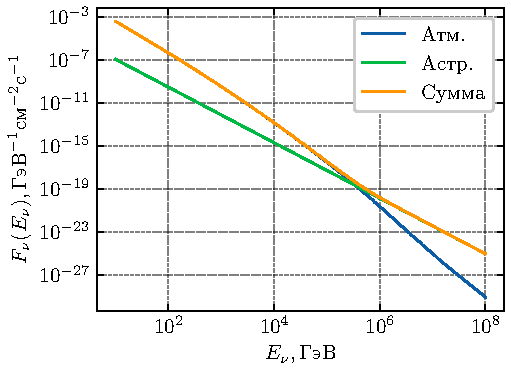
\includegraphics[width=0.8\linewidth]{images/NuProp/fluxes.pdf}
    \caption{Атмосферные и астрофизические нейтринные потоки для мюонного флейвора.}
    \label{NuFluxes_astro_and_atmo}
  \end{figure}
\subsection*{Усреднённое ядро и мантия.}  
В качестве альтернативной гипотезы $H_1$ используется модель с постоянной плотностью $\rho = 8.853~\text{г/см}^3$ в области внутреннего ядра, внешнего ядра и мантии (до радиуса $5600~\text{км}$).  
В остальной части модель совпадает с PREM.  
Для данной пары гипотез ($H_0$, $H_1$) получено значение $\Delta\chi^2 = 6.84$, что соответствует статистической значимости $2.62\sigma$ при одном числе степеней свободы.
  
  \begin{figure}[!h]
    \centering
    \includegraphics[width=0.8\linewidth]{images/NuProp/chi2_rzf_2dxsCT10nlo_PREM_vs_PREM_man_and_ker.png}
    \caption{Распределение статистики $\Delta\chi^2$, полученной при сравнении чисел нейтринных событий для гипотез $H_0$ (модель PREM) и $H_1$ (усреднённые ядро и мантия).}
    \label{NuTom1}
  \end{figure}

Из анализа распределения $\Delta\chi^2$ на рис.~(\ref{NuTom1}) следует, что наибольшая чувствительность нейтринной томографии приходится на диапазон энергий  
\[
E_\nu \sim 10^2\text{–}10^6~\text{ГэВ},
\]
где сечения взаимодействий уже достаточно велики для заметного ослабления потока, но интенсивность ещё не слишком мала.  
Максимум чувствительности наблюдается около $E_\nu \sim 10^4~\text{ГэВ}$.  
Зависимость по углу прихода нейтрино определяется характером альтернативной модели: при изменении плотности в мантии максимум по углу смещается к меньшим значениям $\theta_d$, что отражает различие в эффективных толщинах вещества вдоль траекторий.

\section{Обсуждение и выводы}
\label{sec:conclusions}
В настоящей работе представлены два открытых программных инструмента — \texttt{nudisxs} и \texttt{NuPropagator}, предназначенные для моделирования взаимодействий и распространения нейтрино высоких энергий. 
Первый пакет обеспечивает точное вычисление сечений глубоконеупругого рассеяния на основе современных партонных распределений, 
второй реализует $\mathcal{Z}$-факторный метод, позволяющий учитывать регенерацию нейтрино при прохождении через вещество. 
Оба инструмента ориентированы на применение в нейтринной астрофизике и моделировании детекторов типа IceCube, KM3NeT и Baikal-GVD.

Проведён анализ достоверности партонной модели в диапазоне энергий до $E_\nu \sim 10^9$~ГэВ. 
Показано, что основная неопределённость связана с отсутствием экспериментальных данных в области малых $x \lesssim 10^{-6}$, однако вклад этой области в полное сечение не превышает нескольких процентов. 
Сравнение различных наборов партонных распределений (\texttt{CT10nlo}, \texttt{CT18ZNNLO}, \texttt{nCTEQ15}, \texttt{TUJU19\_nlo}) демонстрирует согласие на уровне $\sim5\%$, что подтверждает надёжность предсказаний в пределах современных феноменологических моделей. 
Таким образом, расчёты нейтринных сечений вплоть до 100 ПэВ энергий можно считать устойчивыми и применимыми для задач астрофизики и нейтринной томографии.

Показано, что учёт регенерации, обусловленной взаимодействиями по нейтральному току, существенно усиливает чувствительность метода нейтринной томографии Земли. 
Без этого эффекта поток нейтрино экспоненциально затухает, тогда как включение регенерации сохраняет измеримый сигнал даже при энергиях $E_\nu \gtrsim 1$~ПэВ. 
Регенерация повышает статистическую значимость наблюдений и открывает возможность реконструкции плотностного профиля ядра по энергетическим спектрам проходящих нейтрино.

Полученные результаты демонстрируют, что крупномасштабные нейтринные телескопы нового поколения (IceCube-Gen2, KM3NeT, Baikal-GVD) смогут использовать потоки астрофизических нейтрино не только как инструмент астрономических наблюдений, но и как физический зонд внутренней структуры Земли. 
Дальнейшее развитие представленных подходов создаёт основу для объединённого анализа данных различных нейтринных обсерваторий, уточнения модели плотности и химического состава земного ядра, а также проверки фундаментальных свойств нейтрино при экстремальных энергиях.

\section*{Благодарности}
Мы выражаем признательность В.~А.~Наумову и К.~С.~Кузьмину за предоставленные материалы и разрешение использовать рисунок~\ref{fig:disxs_compare} в настоящей работе, а также И.~А.~Белолаптикову за полезные обсуждения.
С.~И.~Завьялов выражает благодарность Фонду развития теоретической физики и математики «БАЗИС» за поддержку исследования в рамках гранта № 24-2-10-28-1.
\appendix
\section{Сечения взаимодействия нейтрино}
\subsubsection{Структурные функции и кинематические формулы}
\label{app:structure_functions}

Для случая неполяризованного лептона ненулевыми оказываются следующие функции $A_i$:
\begin{equation}
    \begin{aligned}
        A_1(x, y, E) &= y(xy + a), \\
        A_2(x, y, E) &= 1 - y - \frac{xyM_N}{2E} - \left( \frac{m_{l}}{2E} \right)^2, \\
        A_3(x, y, E) &= y\left( x\left(1 - \frac{y}{2} \right) - \frac{a}{2} \right), \\
        A_4(x, y, E) &= a(xy + a), \\
        A_5(x, y, E) &= -a,
    \end{aligned}
\end{equation}
где $a = m_l^2/(2M_N E)$, а $m_l$ — масса лептона.

В партонной аппроксимации структурные функции выражаются через функции распределения кварков и антикварков:
\begin{equation}
    \begin{aligned}
        F_1(x) &= \frac{1}{2} \sum\limits_{i} e_i^2 \left[ q_i(x) + \bar{q}_i(x) \right], \\
        F_2(x) &= \sum\limits_{i} e_i^2 x \left[ q_i(x) + \bar{q}_i(x) \right], \\
        F_3(x) &= \sum\limits_{i} e_i^2 \left[ q_i(x) - \bar{q}_i(x) \right],
    \end{aligned}
\end{equation}
где $e_i$ — заряд $i$-го кварка в единицах заряда электрона.

Допустимый диапазон квадрата полной массы адронной системы задаётся интервалом $W^2 \in [W^2_{\text{cut}}, W_+^2]$, где $W_{\text{cut}}$ — нижний кинематический порог, а $W_+ = \sqrt{s} - m_l$. При этом пороговая энергия нейтрино равна
\begin{equation}
    E_\nu^{\text{th}} = \frac{(W_{\text{cut}} + m_l)^2 - M_N^2}{2M_N}.
\end{equation}

Допустимая область для переменной Бьёркена $x$ ограничивается значениями:
\begin{equation}
    x^{-}(W_{\text{cut}}) \le x \le x^{+}(W_{\text{cut}}),
\end{equation}
где
\begin{equation}
    x^{\pm}(W_{\text{cut}}) = \frac{a \pm \sqrt{b}}{2c},
\end{equation}
а параметры $a$, $b$, $c$ выражаются через:
\begin{equation}
    \begin{aligned}
        a(W_{\text{cut}}) &= 1 - \frac{[W_{\text{cut}}^2 - M_N^2 - m_l^2][(W_{\text{cut}}^2 - M_N^2)E_\nu + m_l^2 M_N]}{2M_N^2(W_{\text{cut}}^2 - M_N^2)E_\nu^2}, \\
        b(W_{\text{cut}}) &= \left[ 1 - \frac{(W_{\text{cut}} - m_l)^2 - M_N^2}{2M_N E_\nu} \right] \left[ 1 - \frac{(W_{\text{cut}} + m_l)^2 - M_N^2}{2M_N E_\nu} \right], \\
        c(W_{\text{cut}}) &= 1 + \frac{(W_{\text{cut}}^2 - M_N^2 - m_l^2)^2}{4E_\nu^2(W_{\text{cut}}^2 - M_N^2)}.
    \end{aligned}
\end{equation}

После выбора $x$ переменная $y$ выбирается из диапазона:
\begin{equation}
    y^{\text{min}}(E_\nu, W_{\text{cut}}) \le y \le y^+(E_\nu),
\end{equation}
где
\begin{equation}
    \begin{aligned}
        y^{\text{min}}(E_\nu, W_{\text{cut}}) &= \max\left( y^-(E_\nu), y^{\text{cut}}(E_\nu, W_{\text{cut}}) \right), \\
        y^{\text{cut}}(E_\nu, W_{\text{cut}}) &= \frac{W_{\text{cut}}^2 - M_N^2}{2M_N(1 - x)E_\nu},
    \end{aligned}
\end{equation}
и
\begin{equation}
    y^{\pm} = \left[ 1 - \frac{m_l^2}{2E_\nu^2}\left(1 + \frac{E_\nu}{M_N x} \right) \pm \sqrt{ \left(1 - \frac{m_l^2}{2M_N x E_\nu} \right)^2 - \frac{m_l^2}{E_\nu^2} } \right] \left[ 2 + \frac{M_N x}{E_\nu} \right]^{-1}.
\end{equation}

\subsection{Сечение взаимодействия $\overline{\nu}_e e$}

Сечение взаимодействия нейтрино с электроном на три порядка меньше, чем с нуклоном, поэтому из взаимодействий с электроном в нашей работе учитывается только резонанс Глэшоу ($\bar{\nu}_e + e^- \to W^+$). Дифференциальные сечения, используемые в расчётах, приведены по работе~\cite{GANDHI199681}.

Сечение реакции $\bar{\nu}_e e \to \bar{\nu}_e e$:
\begin{equation}
\begin{aligned}
&\frac{d\sigma(\bar{\nu}_e e \to \bar{\nu}_e e)}{dy} 
= \frac{G_F^2 m_e E_\nu}{2\pi} 
    \left[ 
      \frac{R_e^2}{\left(1 + 2m_e E_\nu y / M_Z^2\right)^2} 
    \right] \\
&+ \frac{G_F^2 m_e E_\nu}{2\pi}
    \left[
      \left|
        \frac{L_e}{1 + 2m_e E_\nu y / M_Z^2}
        + \frac{2}{1 - 2m_e E_\nu / M_W^2 + i\,\Gamma_W / M_W}
      \right|^2 (1 - y)^2
    \right],
\end{aligned}
\end{equation}

Сечение реакции $\bar{\nu}_e e \to \bar{\nu}_\mu \mu$:
\begin{equation}
\frac{d\sigma(\bar{\nu}_e e \to \bar{\nu}_\mu \mu)}{dy} 
= \frac{G_F^2 m_e E_\nu}{2\pi} 
   \frac{
     4(1 - y)^2 \left[ 1 - (\mu^2 - m_e^2)/(2 m_e E_\nu) \right]^2
   }{
     \left(1 - 2m_e E_\nu / M_W^2\right)^2 + \Gamma_W^2 / M_W^2
   }.
\end{equation}

Сечение реакции $\bar{\nu}_e e \to \text{адроны})$:
\begin{equation}
\frac{d\sigma(\bar{\nu}_e e \to \text{адроны})}{dy} =
\frac{d\sigma(\bar{\nu}_e e \to \bar{\nu}_\mu \mu)}{dy}
\frac{\Gamma(W \to \text{адроны})}{\Gamma(W \to \mu \bar{\nu}_\mu)},
\end{equation}
где $\Gamma(W \to \text{адроны})$ и $\Gamma(W \to \mu \bar{\nu}_\mu)$ -- ширины распадов $W$ бозона на адроны и $\mu \bar{\nu}_\mu$.
\section{Дополнительные примеры распределений $d^2\sigma/(dx\,dQ^2)$}
\label{sec:examples_extrapolated_region}

Для полноты картины на рис.~(\ref{Pp3}) и~(\ref{Pp6}) приведены примеры дважды дифференциальных нормированных сечений $\frac{1}{\sigma(E_\nu)}\frac{d^2\sigma(E_\nu,x,Q^2)}{dx\,dQ^2}$ для энергий нейтрино $E_\nu = 1$~ТэВ и $1$~ПэВ. 
Рассмотренные распределения иллюстрируют, как с ростом энергии нейтрино максимум функции постепенно смещается в область меньших значений переменной Бьёркена~$x$, что отражает возрастающее значение вклада малых $x$ в полное сечение. 

\begin{figure}[!h]
\centering
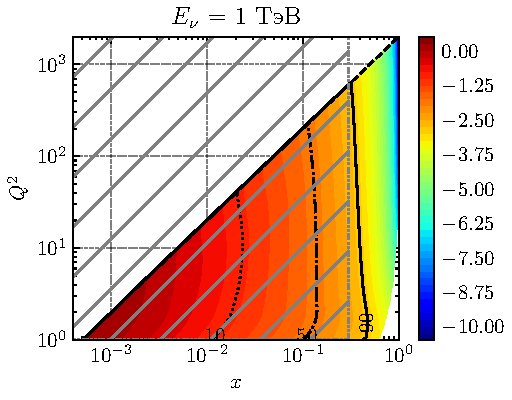
\includegraphics[width=0.8\linewidth]{images/NuProp/cdfxq2_cc_proton_CT18ZNNLO_14_1000.pdf}
\caption{Кумулятивное нормированное сечение $F_{\sigma}(x,Q^2)$ в зависимости от переменных Бьёркена~$x$ и $Q^2$ при энергии нейтрино $E_{\nu} = 1$~ТэВ. Использованы партонные распределения \texttt{CT10nlo}.}
\label{Pp3}
\end{figure}

\begin{figure}[!h]
\centering
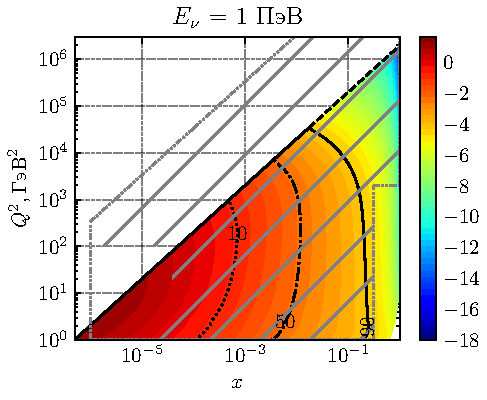
\includegraphics[width=0.8\linewidth]{images/NuProp/cdfxq2_cc_proton_CT18ZNNLO_14_1000000.pdf}
\caption{Кумулятивное нормированное сечение $F_{\sigma}(x,Q^2)$ в зависимости от переменных Бьёркена~$x$ и $Q^2$ при энергии нейтрино $E_{\nu} = 1$~ПэВ. Использованы партонные распределения \texttt{CT10nlo}.}
\label{Pp6}
\end{figure}

Сравнение рисунков показывает, что при увеличении энергии нейтрино до ПэВ-уровня область значимых вкладов смещается в диапазон $x \lesssim 10^{-5}$, подтверждая выводы раздела~\ref{sec:dis_reliability} о растущем влиянии малых~$x$ на формирование полного сечения.

\section{Модель плотности Земли}
\label{sec:prem}
В качестве модели плотности используется модель PREM~\cite{dziewonskiPREM1981}, которая предполагает сферическую симметрию и описывает плотность, давление и другие параметры как функции радиуса. Плотность в модели представлена на рис.~\ref{PREM}.

\begin{figure}[!h]
\centering
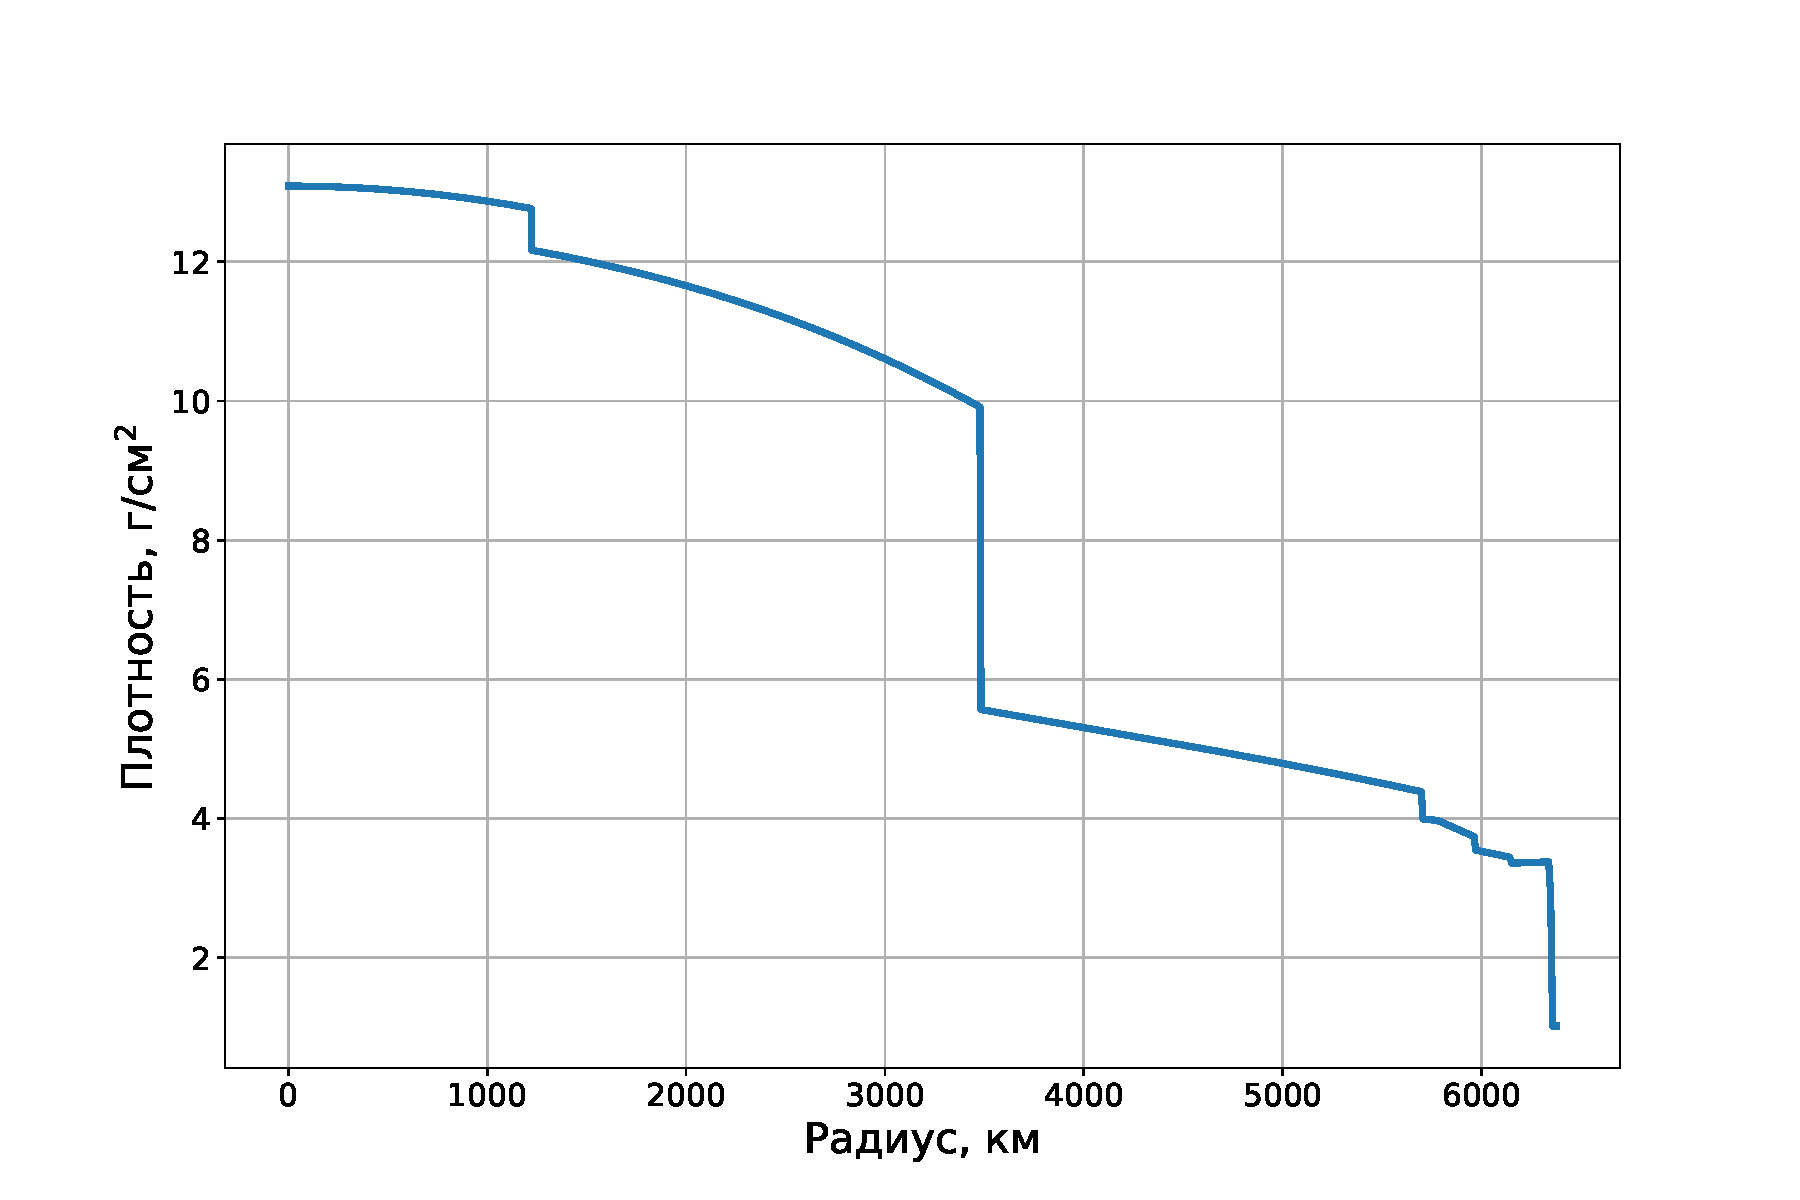
\includegraphics[width=0.8\linewidth]{images/NuProp/PREM.pdf}
\caption{Плотность вещества Земли в модели  PREM.}
\label{PREM}
\end{figure}

\section{Дополнительные примеры чувствительности нейтринной томографии к профилю плотности Земли}
\label{sec:appTomography}

В дополнение к сценарию, рассмотренному в основном тексте, проанализируем ещё два варианта распределения плотности, отличающихся от стандартной модели PREM.  
Для каждого случая вычислены значения статистики $\Delta\chi^2$, характеризующие степень различия с моделью PREM при предположении нейтринного телескопа объёмом $1~\text{км}^3$ и времени наблюдения один год.

\subsection{Усреднённое ядро}

В качестве альтернативной гипотезы $H_1$ рассмотрим модель, в которой плотность вещества принимается постоянной и равной $\rho = 11.87~\text{г/см}^3$ во всей области внутреннего и внешнего ядра, тогда как мантия описывается стандартной моделью PREM.  
Для пары гипотез ($H_0$, $H_1$) получено $\Delta\chi^2 = 0.125$, что соответствует статистической значимости $0.36\sigma$.  
Если увеличить время наблюдения до 25 лет либо использовать нейтринный телескоп существенно большего объёма (например, $30~\text{км}^3$), ожидаемая значимость возрастает до $\sim 2\sigma$.

\begin{figure}[!h]
    \centering
    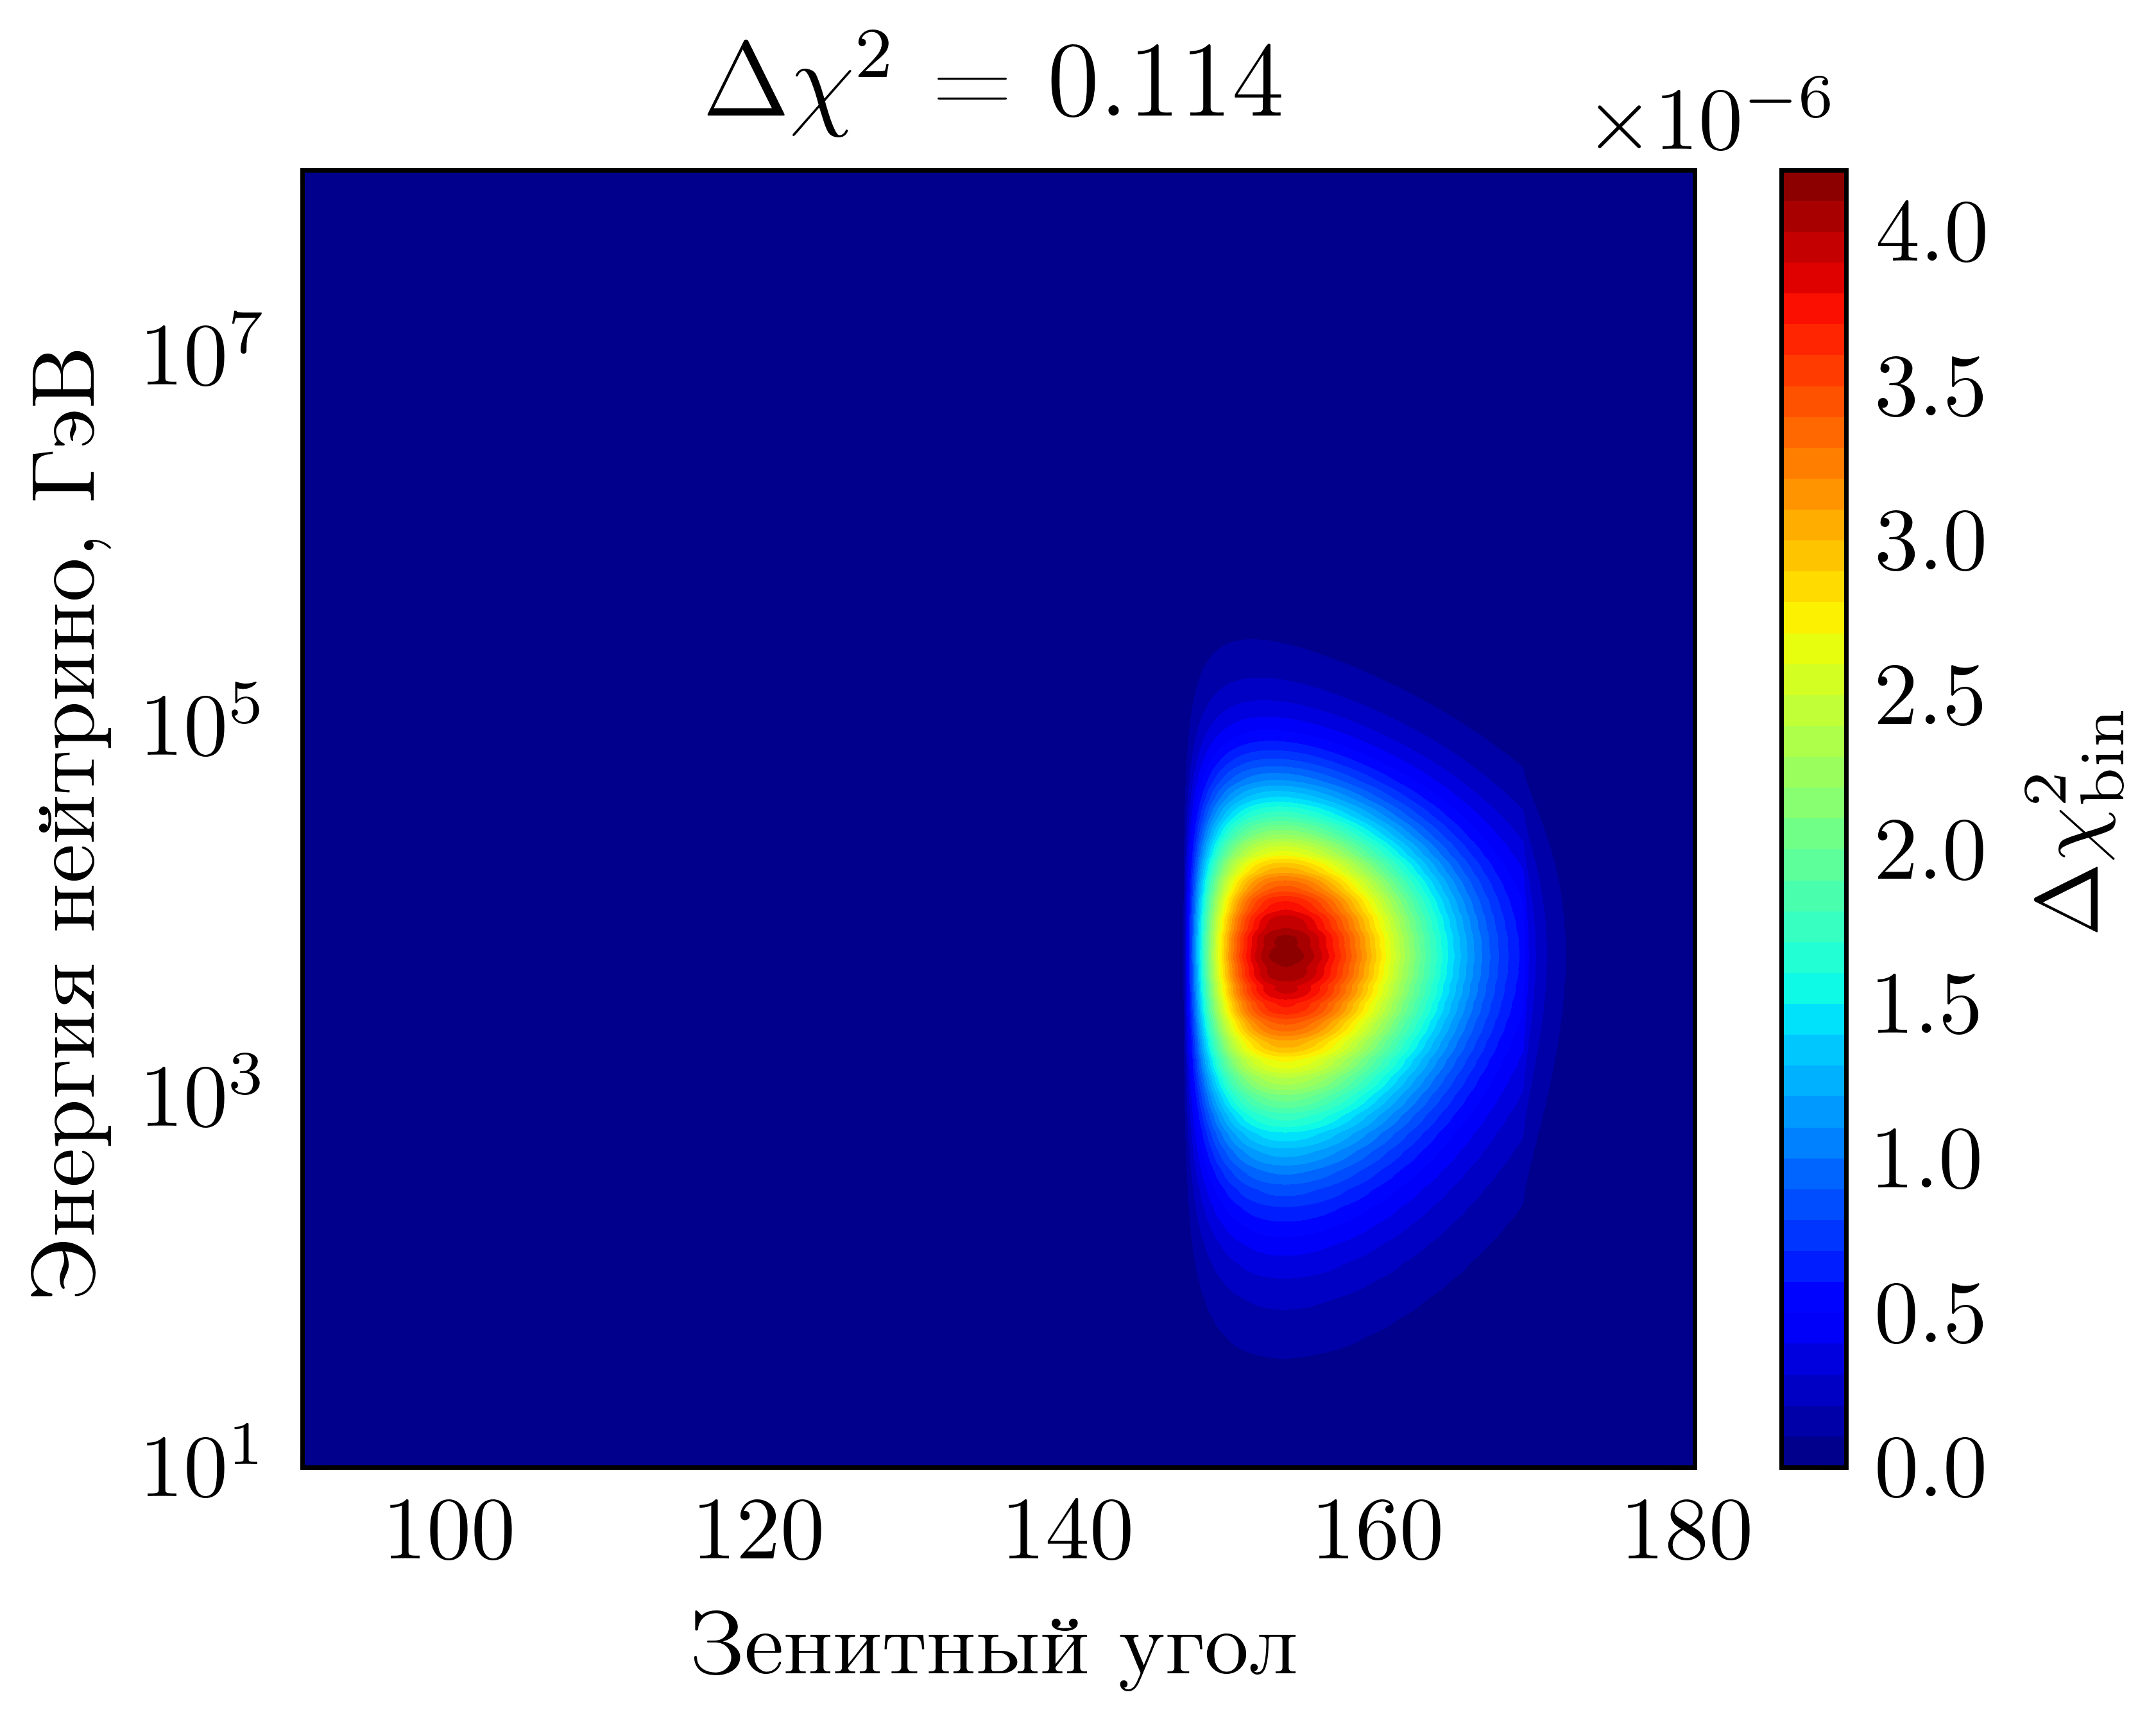
\includegraphics[width=\linewidth]{images/NuProp/chi2_rzf_2dxsCT10nlo_PREM_vs_PREM_av_ext_ker.png}
    \caption{Распределение статистики $\Delta\chi^2$, полученное при сравнении числа нейтринных событий для гипотез $H_0$ (модель PREM) и $H_1$ (усреднённое ядро).}
    \label{NuTom2}
\end{figure}

\subsection{Линейное ядро}

В следующем сценарии в качестве альтернативной гипотезы используется модель, в которой плотность в области внутреннего и внешнего ядра аппроксимируется линейной функцией радиуса.  
Вне ядра распределение плотности совпадает с моделью PREM.  
Для этой пары гипотез ($H_0$, $H_1$) получено $\Delta\chi^2 = 0.665$, что соответствует статистической значимости $0.82\sigma$.  
При увеличении времени наблюдения до десяти лет ожидаемая значимость достигает $\sim 2.8\sigma$.

\begin{figure}[!h]
    \centering
    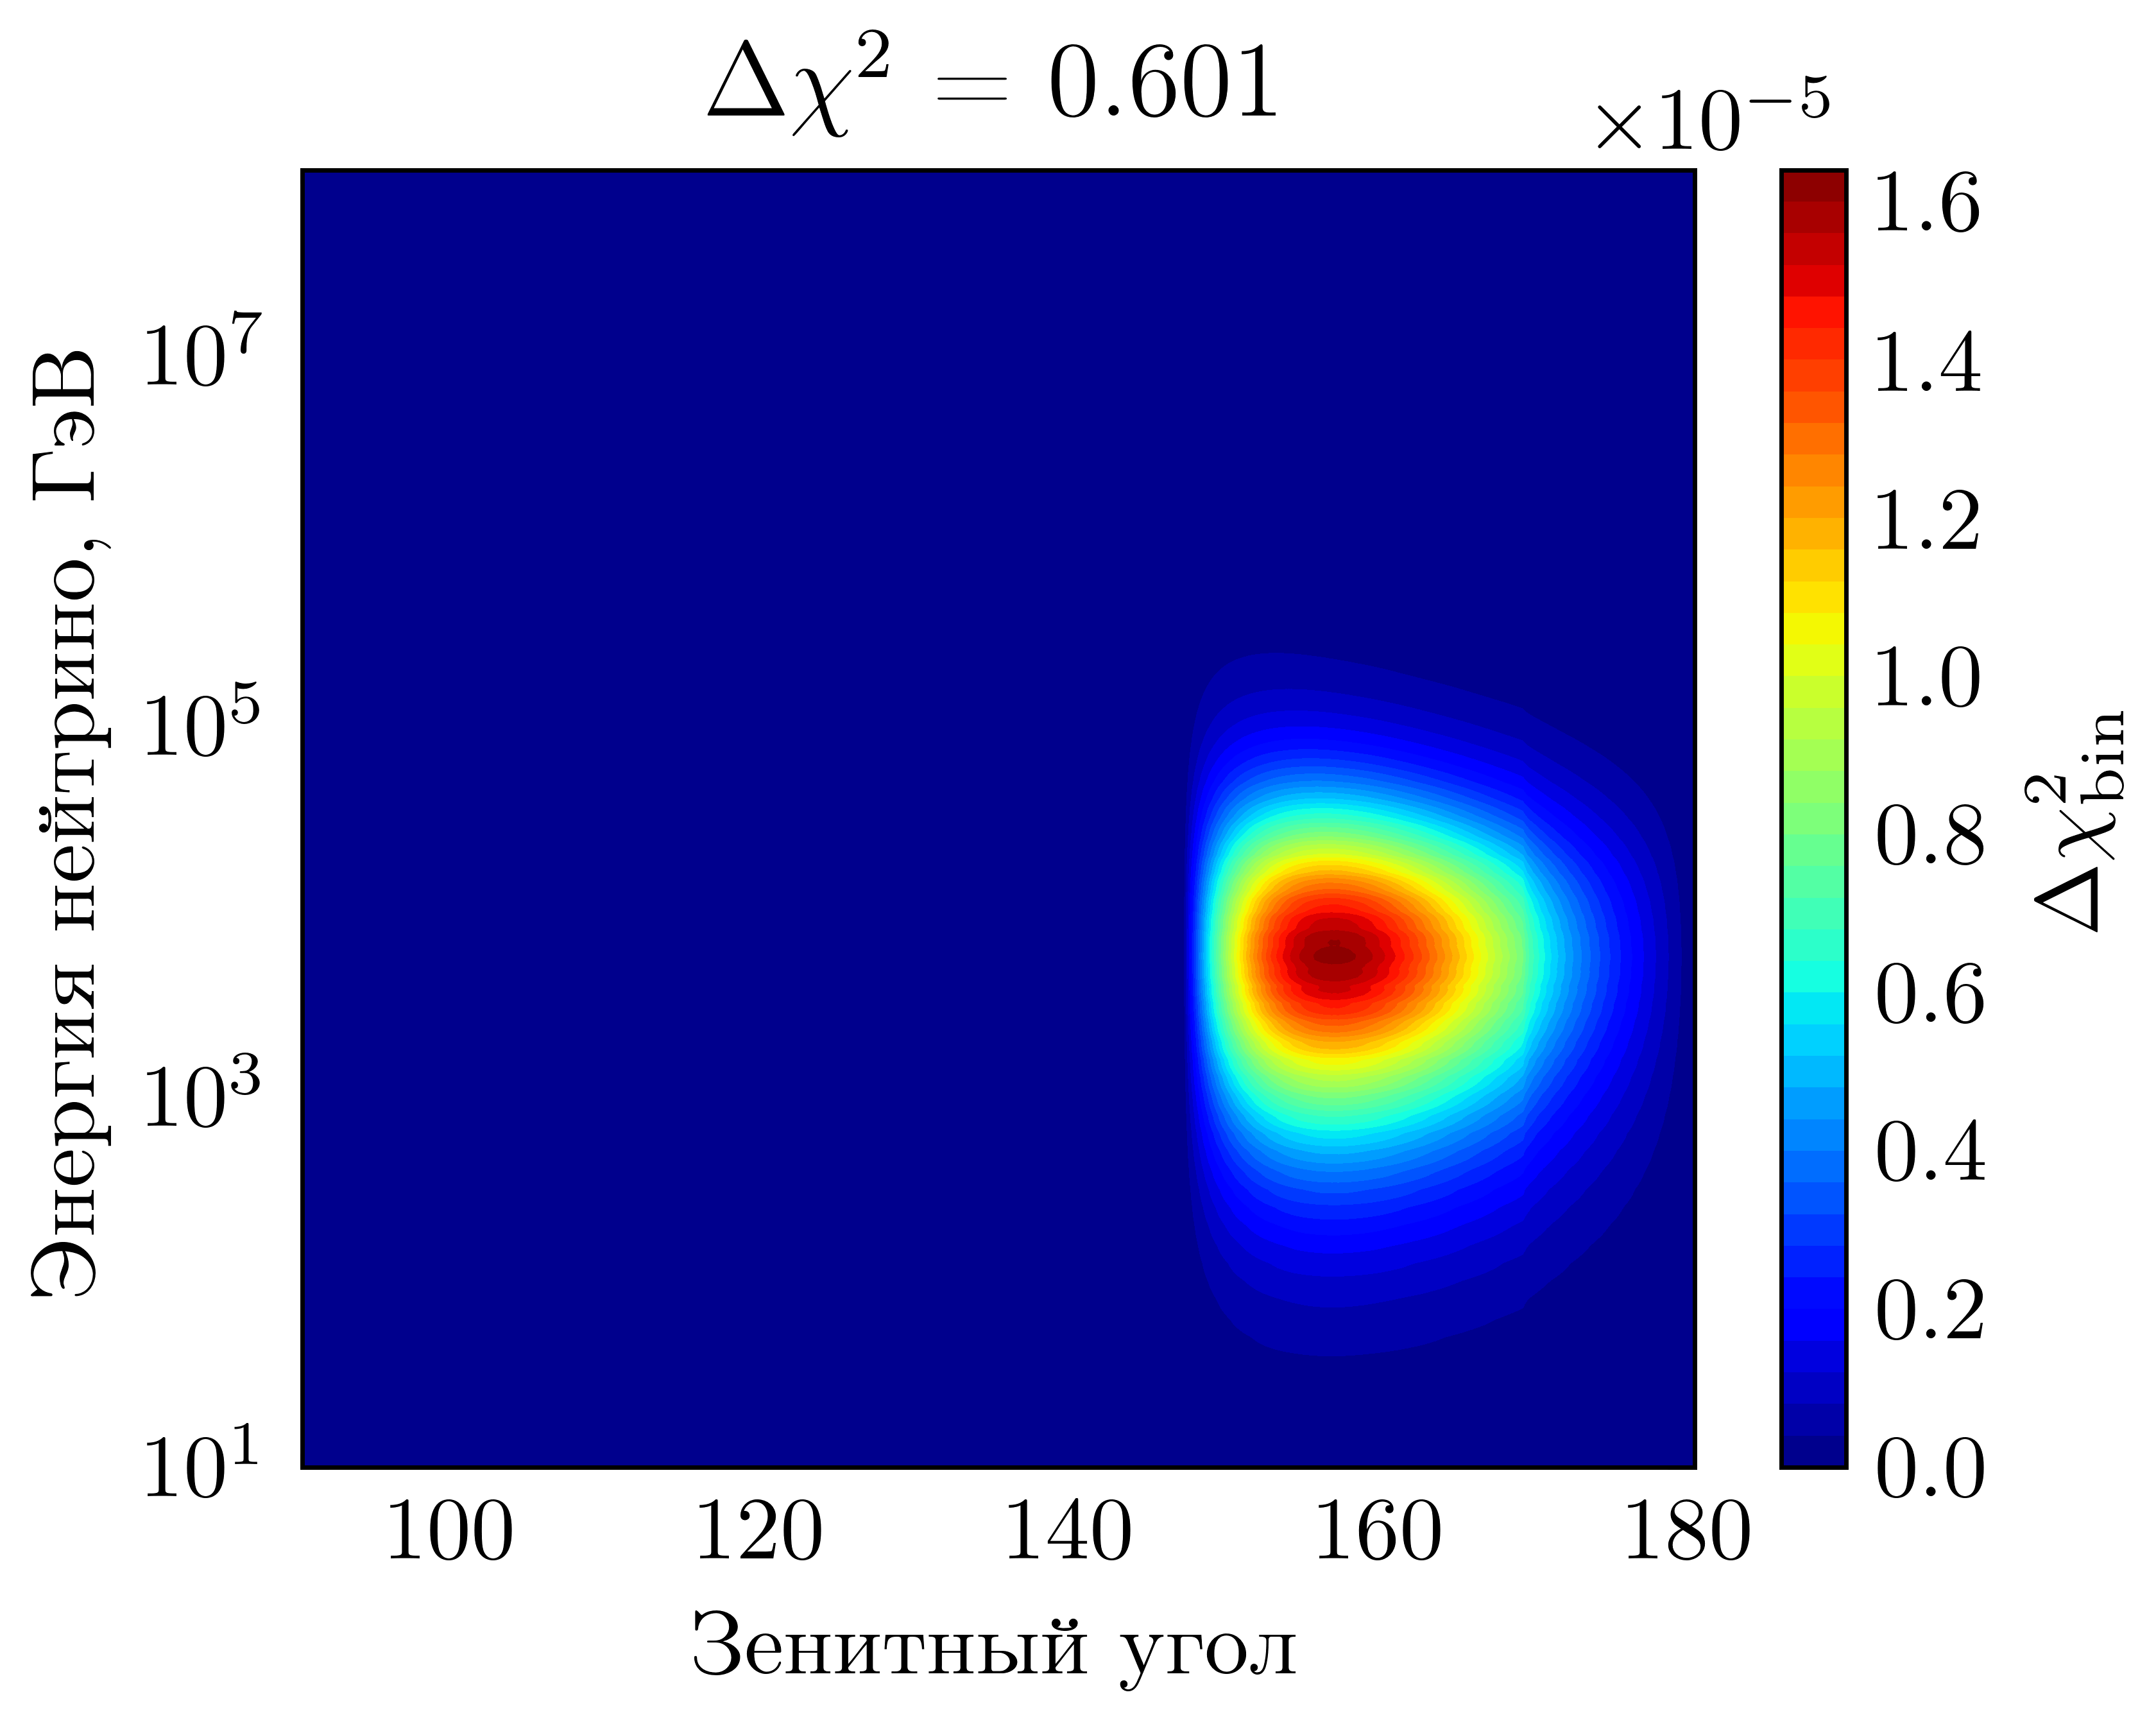
\includegraphics[width=\linewidth]{images/NuProp/chi2_rzf_2dxsCT10nlo_PREM_vs_PREM_lin_ker.png}
    \caption{Распределение статистики $\Delta\chi^2$ для гипотез $H_0$ (модель PREM) и $H_1$ (линейное ядро).}
    \label{NuTom3}
\end{figure}

Полученные результаты демонстрируют, что даже при относительно простых отклонениях от модели PREM метод нейтринной томографии сохраняет чувствительность к изменениям профиля плотности ядра, которая растёт с увеличением статистики и объёма детектора.

% \bibliographystyle{unsrt}
% \bibliography{references}
\printbibliography

\end{document}

Tomography.tex                                                  |  13 ++++++++++---
 appTomography.tex                                               |   6 +++---
 images/NuProp/chi2_rzf_2dxsCT10nlo_PREM_vs_PREM_av.png          | Bin 1154961 -> 238724 bytes
 images/NuProp/chi2_rzf_2dxsCT10nlo_PREM_vs_PREM_av_ext_ker.png  | Bin 1020981 -> 229748 bytes
 images/NuProp/chi2_rzf_2dxsCT10nlo_PREM_vs_PREM_lin_ker.png     | Bin 1067819 -> 234842 bytes
 images/NuProp/chi2_rzf_2dxsCT10nlo_PREM_vs_PREM_man_and_ker.png | Bin 1081373 -> 239860 bytes
 images/NuProp/chi2_rzf_2dxsCT10nlo_PREM_vs_PREM_quad_ker.png    | Bin 1066632 -> 241810 bytes
 images/NuProp/fluxes.pdf                                        | Bin 0 -> 312341 bytes
 references.bib  